% This file serves as the `main' file that includes all of the chapters, 
% appendices, figures, etc.

\listfiles
 %% Changed from 12pt. Fixed dimensions have not been updated.
\documentclass[12pt]{report}

%% Include all packages
% This is a list of packages to include for the main Thesis.
% This file is used by all of the `Chapters', `Appendices', etc.
% Add this file at the beginning of the document.
\newcommand\hmmax{0}
\newcommand\bmmax{0}
\usepackage{acronym}
\usepackage{ae}
\usepackage{aecompl}
\usepackage{afterpage}
\usepackage{amsthm}
\usepackage{amsbsy}
\usepackage{amsfonts}
\usepackage{amsmath}
\usepackage{amssymb}
\usepackage{amstext}
\usepackage{appendix}
\usepackage{array}
\usepackage{authblk}
\usepackage[english]{babel}
\usepackage{blindtext}
\usepackage{bm}
\usepackage{booktabs}
\usepackage{caption}
%\usepackage{CJK}
%\usepackage{ctex}
\usepackage{colortbl}
\usepackage{color}
\usepackage{datetime}
\usepackage{dcolumn}
\usepackage{eepic}
\usepackage{enumitem}
\usepackage{epsfig}
\usepackage{epstopdf}
\usepackage[mathscr]{euscript}
\usepackage{fix-cm}
\usepackage{float}
\usepackage[T1]{fontenc}
\usepackage{footnote}
\usepackage{footmisc}
\usepackage[left=1.5in,right=1in,top=1in,bottom=1in]{geometry}
\usepackage{graphicx}
\usepackage{graphics}
\usepackage[scaled]{helvet}
\usepackage[colorlinks=true,citecolor=blue,linkcolor=blue]{hyperref} % you probably want to make this black for your printed version, but the blue links are nice when working with the pdf
\usepackage[all]{hypcap}
\usepackage{indentfirst}
\usepackage[utf8]{inputenc}
\usepackage{lscape}
\usepackage{listings}
\usepackage{makecell}
\usepackage{makeidx}
\usepackage{mathptmx}
\usepackage{multirow}
\usepackage[round]{natbib}
\usepackage[intoc]{nomencl}
\usepackage{placeins}
\usepackage{relsize}
\usepackage{rotating}
\usepackage{setspace}
\usepackage{soul}
\usepackage{stmaryrd}
\usepackage{subfig}
\usepackage{tabularx}
\usepackage[table, svgnames]{xcolor}
\usepackage[most]{tcolorbox}
\usepackage{textcomp}
\usepackage{threeparttable}
\usepackage{times}
\usepackage{titlesec}
\usepackage{titletoc}
\usepackage[nottoc]{tocbibind}
\usepackage[subfigure, titles]{tocloft}
\usepackage{todonotes}
\usepackage{txfonts}
\usepackage[normalem]{ulem}
\usepackage{units}
\usepackage{url}
\usepackage{xspace}

%% Program-specific configuration
%% You can change the 'pdfkeywords' to whatever your thesis relates to
% PDF settings
\hypersetup{
    pdfauthor=Kyle Godbey,
    pdftitle=Low-Energy Nuclear Reactions Using Time-Dependent Density Functional Theory,
    pdfkeywords={Nuclear Reactions: fusion --- Nuclear Reactions: quasifission --- Nuclear Reactions: transfer --- methods: density functional theory},
    colorlinks=true,
    citecolor=blue,
    linkcolor=black,
    urlcolor=cyan
}


%% Include style files
\usepackage{../Extras/sfchap}
\usepackage{../Extras/sfsection}

%% Include all commands
%%%%%%%%%%%%%%%%%%%%%%%%%%%%%%%%%%%%%%%%%%%%%%%%%%%%%%%%%%%%%%%%%%%%%%%%%%%%%%
%%
%% Macros for TeX/LaTeX documents
%%
%% Author: Victor F. Calderon (http://vcalderon.me)
%%
%%%%%%%%%%%%%%%%%%%%%%%%%%%%%%%%%%%%%%%%%%%%%%%%%%%%%%%%%%%%%%%%%%%%%%%%%%%%%%
%%
%%% This is a list of commands used throughtout the main paper.
%%% Think about them as `aliases', as they can be used for making
%%% the paper look less cluttered.
%%%
%%% Some of these commands were taken from 'Frank C. van den Bosch' macros tex.
%%%
%%% This is a list of commands used throughout the main thesis.
%%% Think about them as `aliases', as they can be used for make the 
%%% thesis less cluttered.
%%%
%%%%%%%%%%%%%%%%%%%%%%%%%%%%%%%%%%%%%%%%%%%%%%%%%%%%%%%%%%%%%%%%%%%%%%%%%%%%%%
%%%%%%%%%%% --- This is where you define your set of commands --- %%%%%%%%%%%%
%%%%%%%%%%%%%%%%%%%%%%%%%%%%%%%%%%%%%%%%%%%%%%%%%%%%%%%%%%%%%%%%%%%%%%%%%%%%%%



%%%%%%%%%%%%%%%%%%%%%%%%%%%%%%%%%%%%%%%%%%%%%%%%%%%%%%%%%%%%%%%%%%%%%%%%%%%%%%
%%%%%%%%%%%%%%%%%%%%%%% ------ Document-specific ------ %%%%%%%%%%%%%%%%%%%%%%
%%%%%%%%%%%%%%%%%%%%%%%%%%%%%%%%%%%%%%%%%%%%%%%%%%%%%%%%%%%%%%%%%%%%%%%%%%%%%%

\renewcommand{\nomname}{LIST OF ABBREVIATIONS}

% New command: caption for name
\newcommand\tline[2]{$\underset{\text{#1}}{\text{\underline{\hspace{#2}}}}$}

%%%%%%%%%%%%%%%%%%%%%%%%%%%%%%%%%%%%%%%%%%%%%%%%%%%%%%%%%%%%%%%%%%%%%%%%%%%%%%
%%%%%%%%%%%%%%%%%%%%%%% ------ Paper-specific ------ %%%%%%%%%%%%%%%%%%%%%%%%%
%%%%%%%%%%%%%%%%%%%%%%%%%%%%%%%%%%%%%%%%%%%%%%%%%%%%%%%%%%%%%%%%%%%%%%%%%%%%%%

% -- Paper sections

% -- Citations
\newcommand{\etal}{\emph{et al.}}
\providecommand{\eprint}[1]{\href{http://arxiv.org/abs/#1}{#1}}

% -- Text
\def\rma{{\rm a}}
\def\rmb{{\rm b}}
\def\rmc{{\rm c}}
\def\rmd{{\rm d}}
\def\rme{{\rm e}}
\def\rmf{{\rm f}}
\def\rmg{{\rm g}}
\def\rmh{{\rm h}}
\def\rmi{{\rm i}}
\def\rmj{{\rm j}}
\def\rmk{{\rm k}}
\def\rml{{\rm l}}
\def\rmm{{\rm m}}
\def\rmn{{\rm n}}
\def\rmo{{\rm o}}
\def\rmp{{\rm p}}
\def\rmq{{\rm q}}
\def\rmr{{\rm r}}
\def\rms{{\rm s}}
\def\rmt{{\rm t}}
\def\rmu{{\rm u}}
\def\rmv{{\rm v}}
\def\rmw{{\rm w}}
\def\rmx{{\rm x}}
\def\rmy{{\rm y}}
\def\rmz{{\rm z}}

\def\rmA{{\rm A}}
\def\rmB{{\rm B}}
\def\rmC{{\rm C}}
\def\rmD{{\rm D}}
\def\rmE{{\rm E}}
\def\rmF{{\rm F}}
\def\rmG{{\rm G}}
\def\rmH{{\rm H}}
\def\rmI{{\rm I}}
\def\rmJ{{\rm J}}
\def\rmK{{\rm K}}
\def\rmL{{\rm L}}
\def\rmM{{\rm M}}
\def\rmN{{\rm N}}
\def\rmO{{\rm O}}
\def\rmP{{\rm P}}
\def\rmQ{{\rm Q}}
\def\rmR{{\rm R}}
\def\rmS{{\rm S}}
\def\rmT{{\rm T}}
\def\rmU{{\rm U}}
\def\rmV{{\rm V}}
\def\rmW{{\rm W}}
\def\rmX{{\rm X}}
\def\rmY{{\rm Y}}
\def\rmZ{{\rm Z}}

\def\calA{{\cal A}}
\def\calB{{\cal B}}
\def\calC{{\cal C}}
\def\calD{{\cal D}}
\def\calE{{\cal E}}
\def\calF{{\cal F}}
\def\calG{{\cal G}}
\def\calH{{\cal H}}
\def\calI{{\cal I}}
\def\calJ{{\cal J}}
\def\calK{{\cal K}}
\def\calL{{\cal L}}
\def\calM{{\cal M}}
\def\calN{{\cal N}}
\def\calO{{\cal O}}
\def\calP{{\cal P}}
\def\calQ{{\cal Q}}
\def\calR{{\cal R}}
\def\calS{{\cal S}}
\def\calT{{\cal T}}
\def\calU{{\cal U}}
\def\calV{{\cal V}}
\def\calW{{\cal W}}
\def\calX{{\cal X}}
\def\calY{{\cal Y}}
\def\calZ{{\cal Z}}

\def\ba{{\bf a}}
\def\bb{{\bf b}}
\def\bc{{\bf c}}
\def\bd{{\bf d}}
\def\be{{\bf e}}
\def\bff{{\bf f}}
\def\bg{{\bf g}}
\def\bh{{\bf h}}
\def\bi{{\bf i}}
\def\bj{{\bf j}}
\def\bk{{\bf k}}
\def\bl{{\bf l}}
\def\bm{{\bf m}}
\def\bn{{\bf n}}
\def\bo{{\bf o}}
\def\bp{{\bf p}}
\def\bq{{\bf q}}
\def\br{{\bf r}}
\def\bs{{\bf s}}
\def\bt{{\bf t}}
\def\bu{{\bf u}}
\def\bv{{\bf v}}
\def\bw{{\bf w}}
\def\bx{{\bf x}}
\def\by{{\bf y}}
\def\bz{{\bf z}}

\def\bA{{\bf A}}
\def\bB{{\bf B}}
\def\bC{{\bf C}}
\def\bD{{\bf D}}
\def\bE{{\bf E}}
\def\bF{{\bf F}}
\def\bG{{\bf G}}
\def\bH{{\bf H}}
\def\bI{{\bf I}}
\def\bJ{{\bf J}}
\def\bK{{\bf K}}
\def\bL{{\bf L}}
\def\bM{{\bf M}}
\def\bN{{\bf N}}
\def\bO{{\bf O}}
\def\bP{{\bf P}}
\def\bQ{{\bf Q}}
\def\bR{{\bf R}}
\def\bS{{\bf S}}
\def\bT{{\bf T}}
\def\bU{{\bf U}}
\def\bV{{\bf V}}
\def\bW{{\bf W}}
\def\bX{{\bf X}}
\def\bY{{\bf Y}}
\def\bZ{{\bf Z}}

%%%%%%%%%%%%%%%%%%%%%%%%%%%%%%%%%%%%%%%%%%%%%%%%%%%%%%%%%%%%%%%%%%%%%%%%%%%%%%
%%%%%%%%%%%%%%%%%%%%%%% ------ Project-specific ------ %%%%%%%%%%%%%%%%%%%%%%%
%%%%%%%%%%%%%%%%%%%%%%%%%%%%%%%%%%%%%%%%%%%%%%%%%%%%%%%%%%%%%%%%%%%%%%%%%%%%%%

\newcommand{\BDM}{{\tt BDM$\,$}}
\newcommand{\Rockstar}{{\tt ROCKSTAR$\,$}}
\newcommand{\Subfind}{{\tt SUBFIND$\,$}}
\newcommand{\SURV}{{\tt SURV$\,$}}
\newcommand{\HBT}{{\tt HBT$\,$}}
\newcommand{\bfof}{\texttt{berlind-fof}\xspace}
\newcommand{\MPA}{MPA-JHU }

%%%%%%%%%%%%%%%%%%%%%%%%%%%%%%%%%%%%%%%%%%%%%%%%%%%%%%%%%%%%%%%%%%%%%%%%%%%%%%
%%%%%%%%%%%%%%%%%%%%%%% ------ Figure-specific ------ %%%%%%%%%%%%%%%%%%%%%%%%
%%%%%%%%%%%%%%%%%%%%%%%%%%%%%%%%%%%%%%%%%%%%%%%%%%%%%%%%%%%%%%%%%%%%%%%%%%%%%%

\newcommand{\figwidth}{0.47}
\newcommand{\figheight}{0.80}

%%%%%%%%%%%%%%%%%%%%%%%%%%%%%%%%%%%%%%%%%%%%%%%%%%%%%%%%%%%%%%%%%%%%%%%%%%%%%%
%%%%%%%%%%%%%%%%%%%%%%% ------ Math-related ------ %%%%%%%%%%%%%%%%%%%%%%%%%%%
%%%%%%%%%%%%%%%%%%%%%%%%%%%%%%%%%%%%%%%%%%%%%%%%%%%%%%%%%%%%%%%%%%%%%%%%%%%%%%

\def\beq{\begin{equation}}
\def\eeq{\end{equation}}
\def\barray{\begin{eqnarray}}
\def\earray{\end{eqnarray}}
\def\beqarray{\begin{eqnarray}}
\def\eeqarray{\end{eqnarray}}

% - Less than approximate and all that
\def\gtsima{$\; \buildrel > \over \sim \;$}
\def\ltsima{$\; \buildrel < \over \sim \;$}
\def\prosima{$\; \buildrel \propto \over \sim \;$}
\def\gsim{\lower.7ex\hbox{\gtsima}}
\def\lsim{\lower.7ex\hbox{\ltsima}}
\def\simgt{\lower.7ex\hbox{\gtsima}}
\def\simlt{\lower.7ex\hbox{\ltsima}}
\def\simpr{\lower.7ex\hbox{\prosima}}
\def\la{\lsim}
\def\ga{\gsim}
\def\lta{\la}
\def\gta{\ga}

% - Special Math symbols
\def\tensor{\sf}
\newcommand{\tomega}{\widetilde{\omega}}

%%%%%%%%%%%%%%%%%%%%%%%%%%%%%%%%%%%%%%%%%%%%%%%%%%%%%%%%%%%%%%%%%%%%%%%%%%%%%%
%%%%%%%%%%%%%%%%%%%%%%% ------ Draft-editing ------ %%%%%%%%%%%%%%%%%%%%%%%%%%
%%%%%%%%%%%%%%%%%%%%%%%%%%%%%%%%%%%%%%%%%%%%%%%%%%%%%%%%%%%%%%%%%%%%%%%%%%%%%%

\newcommand{\ab}[1]{{\color{blue}{\bf AB:} #1}}
\newcommand{\vc}[1]{{\color{cyan}{\bf VC:} #1}}
\newcommand{\XXX}[2]{{\sf #1}}
\newcommand{\QQQ}[1]{{\sc $<$#1$>$}}

%% For the 'changes' package
\setstcolor{red}
\definecolor{orange}{rgb}{1,0.5,0}
\setlength{\marginparwidth}{3cm}
\newcommand{\note}[2][]{}

%%%%%%%%%%%%%%%%%%%%%%%%%%%%%%%%%%%%%%%%%%%%%%%%%%%%%%%%%%%%%%%%%%%%%%%%%%%%%%
%%%%%%%%%%%%%%%%%%%%%%% ------ Hyperlinks ------ %%%%%%%%%%%%%%%%%%%%%%%%%%%%%
%%%%%%%%%%%%%%%%%%%%%%%%%%%%%%%%%%%%%%%%%%%%%%%%%%%%%%%%%%%%%%%%%%%%%%%%%%%%%%

\newcommand*{\mailto}[1]{\href{mailto:#1}{#1}}
\newcommand*{\http}[1]{\href{http://#1}{#1}}
\newcommand*{\https}[1]{\href{https://#1}{#1}}

%%%%%%%%%%%%%%%%%%%%%%%%%%%%%%%%%%%%%%%%%%%%%%%%%%%%%%%%%%%%%%%%%%%%%%%%%%%%%%
%%%%%%%%%%%%%%%%%%%%%%% ------ Astrophysics-specific ------ %%%%%%%%%%%%%%%%%%
%%%%%%%%%%%%%%%%%%%%%%%%%%%%%%%%%%%%%%%%%%%%%%%%%%%%%%%%%%%%%%%%%%%%%%%%%%%%%%

% - Within equation
\newcommand{\kmsmpc}{\>{\rm km}\,{\rm s}^{-1}\,{\rm Mpc}^{-1}}
\newcommand{\kms}{\>{\rm km}\,{\rm s}^{-1}}
\newcommand{\pc}{\>{\rm pc}}
\newcommand{\cm}{\>{\rm cm}}
\newcommand{\Gpc}{\>{\rm Gpc}}
\newcommand{\Mpc}{\>{\rm Mpc}}
\newcommand{\kpc}{\>{\rm kpc}}
\newcommand{\Msun}{\>{\rm M_{\odot}}}
\newcommand{\Lsun}{\>{\rm L_{\odot}}}
\newcommand{\MLsun}{\>({\rm M}/{\rm L})_{\odot}}
\newcommand{\Mbh}{M_{\bullet}}
\newcommand{\Vrot}{V_{\rm rot}}
\newcommand{\Vmax}{V_{\rm max}}
\newcommand{\Vvir}{V_{\rm vir}}
\newcommand{\Vrat}{V_{\rm max}/V_{{\rm vir},0}}
\newcommand{\mtol}{\>{\rm (M/L)_{\odot}}}
\newcommand{\erg}{\>{\rm erg}}
\newcommand{\kpch}{\>{h^{-1}{\rm kpc}}}
\newcommand{\mpch}{\>h^{-1}{\rm {Mpc}}}
\newcommand{\yr}{\>{\rm yr}}
\newcommand{\yrs}{\>{\rm yrs}}
\newcommand{\Msunh}{\>h^{-1}\rm M_\odot}
\newcommand{\Lsunh}{\>h^{-2}\rm L_\odot}
\newcommand{\wcalN}{\tilde{{\cal N}}}
\newcommand{\walpha}{\tilde{\alpha}}
\newcommand{\wLstar}{\tilde{L}^{*}}
\newcommand{\hxi}{\hat{\xi}}
\newcommand{\lcdm}{{\ensuremath{\Lambda}CDM}\xspace}
\newcommand{\vcir}{V_{\rm c}}
\newcommand{\vh}{V_{\rm c}}
\newcommand{\Obaryon}{{\Omega_{\rm B,0}}}
\newcommand{\Kdegree}{\>{\rm K}}
\newcommand{\keV}{\>{\rm keV}}
\newcommand{\Vhalo}{V_{\rm c}}
\newcommand{\Mhalo}{M_{\rm h}}
\newcommand{\Tvir}{T_{\rm vir}}
\newcommand{\vesc}{V_{\rm esc}}
\newcommand{\Lya}{{\rm Ly}\alpha}
\newcommand{\msunh}{\>h^{-1}\rm M_\odot}
\newcommand{\Lsunhh}{\,h^{-2}\rm L_\odot}
\newcommand{\avg}[1]{\langle #1 \rangle}
\newcommand{\avglogm}{\avg{\log M}(L_c)}
\newcommand{\avgloglc}{\avg{\log L_c}(M)}
\newcommand{\siglogm}{\avg{\sigma_{\log M}}(L_c)}
\newcommand{\ploglcm}{P(\log L_c|M)}
\newcommand{\plogmlc}{P(\log M|L_c)}
\newcommand{\sigc}{\sigma_{{\rm ln} c}}
\newcommand{\drm}{{\rm d}}
\newcommand{\ombh}{\>\Omega_{\rm b}\,h^{2}}
\newcommand{\bolds}[1]{{\bf #1}}
\newcommand{\mgroup}{\ensuremath{M_\textrm{group}}\xspace}
\newcommand{\mcf}{\ensuremath{\mathcal{M}(r_{p})}\xspace}
\newcommand{\mcft}{\texorpdfstring{\mcf}{MCF}}
\newcommand{\dsum}{\displaystyle \sum\limits}

% - Outside equation
\newcommand{\msun}{h^{-1}M_\odot}
\newcommand{\hkpc}{\mbox{$h^{-1}\textrm{kpc}$}}
\newcommand{\hmpc}{\mbox{$h^{-1}\textrm{Mpc}$} }
\newcommand{\kmsMpc}{\mbox{$\textrm{km}\ \textrm{s}^{-1}\ \textrm{Mpc}^{-1}$}}
\newcommand{\hmpcthreeinv}{\mbox{$h^{3} \textrm{Mpc}^{-3}$}}
\newcommand{\mstar}{\mbox{$\textrm{M}_{\star}$}}
\newcommand{\gr}{\ensuremath{(g-r)}\xspace}
\newcommand{\ssfr}{{sSFR}\xspace}
\newcommand{\sfr}{{SFR}\xspace}
\newcommand{\logssfr}{$\log\ \textrm{sSFR}$}
\newcommand{\sersic}{{S\'ersic}\xspace}
\newcommand{\xirp}{$\xi(r_{p})$}
\newcommand{\rband}{\textit{r}-band}
\newcommand{\gband}{\textit{g}-band }
\newcommand{\lamA}{${\Lambda}30/90 \, $}
\newcommand{\lamC}{${\Lambda}25/75 \, $}
\newcommand{\lamD}{${\Lambda}20/65 \, $}
\newcommand{\lamB}{${\Lambda}30/65 \, $}

% - Galaxy Samples
\newcommand{\MD}[1]{{\texttt Mr#1-SDSS}\xspace}
\newcommand{\MM}[1]{{\texttt Mr#1-Mock}\xspace}
\newcommand{\MR}[1]{{\texttt Mr#1}\xspace}
\newcommand{\Mr}[1]{{Mr#1}\xspace}

%%%%%%%%%%%%%%%%%%%%%%%%%%%%%%%%%%%%%%%%%%%%%%%%%%%%%%%%%%%%%%%%%%%%%%%%%%%%%%
%%%%%%%%%%%%%%%%%%%%%%% ------ Notes, comments, etc. ------ %%%%%%%%%%%%%%%%%%
%%%%%%%%%%%%%%%%%%%%%%%%%%%%%%%%%%%%%%%%%%%%%%%%%%%%%%%%%%%%%%%%%%%%%%%%%%%%%%




%% Include Headings settings
% These are the settings for the `Chapters', `Sections', etc.
% To generate the final document, run latex, build and quick build commands
% on the skeleton-thesis file not this one.

%%%%%%%%%%%%%%%%%%%%%%%%%%%%%%%%%%%%%%%%%%%%%%%%%%%%%%%%%%%%%%%%%%%%%%%%%%%%%
%%%%%%%%%%% --- List of Settings for the main Thesis document --- %%%%%%%%%%%
%%%%%%%%%%%%%%%%%%%%%%%%%%%%%%%%%%%%%%%%%%%%%%%%%%%%%%%%%%%%%%%%%%%%%%%%%%%%%

%%
%% Page Settings
\textwidth=6in \oddsidemargin=0.5in \topmargin=-0.5in
\textheight=9in  % 9in must include page numbers
\textfloatsep = 0.4in
\addtocontents{toc}{\vspace{0.4in} \hfill
Page\endgraf} \addtocontents{lof}{\vspace{0.2in} \hspace{0.13in} \
Figure\hfill Page\endgraf} \addtocontents{lot}{\vspace{0.2in}
\hspace{0.13in} \ Table\hfill Page\endgraf}

%%
%% Graphics and Figures
\graphicspath{ {../Figures/}}
\DeclareGraphicsExtensions{.pdf, .jpeg, .png, .PNG, .eps, .tiff}

%%
%% URLs and Links
\urlstyle{same}

%%
%% Table of Contents
\setcounter{secnumdepth}{7}
\setcounter{tocdepth}{1}
\renewcommand{\contentsname}{TABLE OF CONTENTS}
\renewcommand{\listfigurename}{LIST OF FIGURES}
\renewcommand{\listtablename}{LIST OF TABLES}
\renewcommand{\bibname}{\texorpdfstring{{BIBLIOGRAPHY\vspace{10mm}}}{BIBLIOGRAPHY}}

%%
%% Stats Table label
\newcommand{\statslabel}[2]{\multirowcell{#1}[-1.6mm][c]{#2}}

%%
%% Below heading rule
\newcommand{\otoprule}{\midrule[\heavyrulewidth]}

%%
%% Prevent double spaced equations
\newenvironment{tightequation}{\singlespace\begin{equation}}{\end{equation}}

%%
%% Extra junk to pretty up the table of contents
\setlength{\cftsecnumwidth}{2.8em}
\setlength{\cftsubsecnumwidth}{3.7em}
\setlength{\cftsubsubsecnumwidth}{4.6em}
\setlength{\cftparanumwidth}{5.5em}
\setlength{\cftsubparanumwidth}{6.5em}
\setlength{\cfttabnumwidth}{3.5em}
\setlength{\cftfignumwidth}{3.5em} 

%%
%% Chapter Mark
\renewcommand{\chaptermark}[1]{%
  \markboth{\MakeUppercase{%
      \chaptername}\ \thechapter.%
    \ #1}{}}

%%%%%%%%%%%%%%%%%%%%%%%%%%%%%%%%%%%%%%%%%%%%%%%%%%%%%%%%%%%%%%%%%%%%%%%%%%%%%%
%%%%%%%%%%%%%%%%%%% ------ Chapter and Section format ------ %%%%%%%%%%%%%%%%%
%%%%%%%%%%%%%%%%%%%%%%%%%%%%%%%%%%%%%%%%%%%%%%%%%%%%%%%%%%%%%%%%%%%%%%%%%%%%%%

%%
%% These commands will change the sections and chapter format to arabic and
%% not roman numerals.

\renewcommand{\thechapter}{\arabic{chapter}}
\renewcommand{\thesection}{\arabic{chapter}.\arabic{section}}
\renewcommand{\thefigure}{\arabic{chapter}.\arabic{figure}}
\renewcommand{\thetable}{\arabic{chapter}.\arabic{table}}


%% Add citation aliases if applicable
% \defcitealias{citation_key}{citation_alias}

%% Starting documents
\begin{document}

%%
%% Title page
% This is an example for a `Title Page'.
% To generate the final document, run latex, build and quick build commands
% on the skeleton-thesis file not this one.

%%% Options for signature
\newtoggle{signatures}
\IfSubStr{ n }{y}{ \toggletrue{signatures} }{ \togglefalse{signatures} }

%% Starting `Title Page'

% This setting will make a difference to the output because the page number is
% suppressed for the title page.
\pagenumbering{alph}

%% Adding metadata for title page
\begin{titlepage}
\thispagestyle{empty}\enlargethispage{\the\footskip}
\begin{center}
    {\setstretch{1.66} { LOW-ENERGY NUCLEAR REACTIONS USING TIME-DEPENDENT DENSITY FUNCTIONAL THEORY }\par}
    \vskip .4in
    By
    \vskip .3in
    { Kyle Godbey }
    \vskip .3in

    \begin{doublespace}
    Dissertation\\
        Submitted to the Faculty of the           \\
        Graduate School of Vanderbilt University  \\
        in partial fulfillment of the requirements\\
        for the degree of \\ [.1in]
    \end{doublespace}
    \MakeUppercase{DOCTOR OF PHILOSOPHY} \\[.1in]
    in \\ [.1in]
    { Physics }  \\ [.25in]
    { May 8$^{\mathrm{th}}$, 2020 }\\ [.25in]
    Nashville, Tennessee
    \vskip .5in
\end{center}

%%%%% --- Committee Members - Signatures --- %%%%%
\iftoggle{signatures}{
    \noindent \hskip 0.1in Approved: \hskip 3.35in  Date: \\[2.0em]
    \noindent\begin{tabular}{ll}
        % Member 1
        \makebox[4.0in]{\hrulefill} & \makebox[1.5in]{\hrulefill}\\
        Victoria Greene, Ph.D. & \\[0.15in]
        % Member 2
        \makebox[4.0in]{\hrulefill} & \makebox[1.5in]{\hrulefill}\\
        Kelly Holley-Bockelmann, Ph.D. & \\[0.15in]
        % Member 3
        \makebox[4.0in]{\hrulefill} & \makebox[1.5in]{\hrulefill}\\
        Norman Tolk, Ph.D. & \\[0.15in]
        % Member 4
        \makebox[4.0in]{\hrulefill} & \makebox[1.5in]{\hrulefill}\\
        Sait A. Umar, Ph.D. & \\[0.15in]
        % Member 5
        \makebox[4.0in]{\hrulefill} & \makebox[1.5in]{\hrulefill}\\
        Kalman Varga, Ph.D. & \\[0.15in]
    \end{tabular}
}{
    \begin{center}
        \begin{doublespace}
            Approved:\\
            % 1st Committee Member
            Victoria Greene, Ph.D.\\[.14in]
            % 2nd Committee Member
            Kelly Holley-Bockelmann, Ph.D.\\[.14in]
            % 3rd Committee Member
            Norman Tolk, Ph.D.\\[.14in]
            % 4th Committee Member
            Sait A. Umar, Ph.D.\\[.14in]
            % 5th Committee Member
            Kalman Varga, Ph.D.\\[.14in]
        \end{doublespace}
    \end{center}
}

\end{titlepage}


%% This setting will make a difference to the output because the page number
%% is suppressed for the title.
\pagenumbering{alph}

% Changing page numbering style
\doublespacing
\pagenumbering{roman} \setcounter{page}{2}

%%
%% Dedication
% This is an example of the `Dedication' section.
% To generate the final document, run latex, build and quick build commands
% on the skeleton-thesis file (not this one)

\chapter*{DEDICATION}\label{dedication}
\addcontentsline{toc}{chapter}{DEDICATION}
\vspace{7mm}

\begin{center}

\vspace{80mm}

%I dedicate this thesis

\vspace{7mm}

%To my Family,

\vspace{7mm}

%with their ever present light

\vspace{7mm}

%And my Friends,

\vspace{7mm}




    
\end{center}

%%
%% Acknowledgements
% This is an example of the `Acknowledgment' section.
% To generate the final document, run latex, build and quick build commands
% on the skeleton-thesis file (not this one)

\chapter*{Acknowledgment}\label{acknowledgment}
\addcontentsline{toc}{chapter}{ACKNOWLEDGMENTS}
\vspace{7mm}

First and foremost, ...


%% Spacing settings
\singlespacing

%%
%% Table of contents
\tableofcontents

%%
%% List of Tables
\begingroup
\setlength{\parskip}{1\baselineskip}
\listoftables
\newpage

%%
%% List of figures
\listoffigures
\newpage
\endgroup

%%
%% Back to arabic page numbering
\normalsize
\doublespacing
\pagenumbering{arabic}
\setcounter{page}{1}

%%
%% Adding extra 'CHAPTER' to table of contents
\cftaddtitleline{toc}{chapter}{CHAPTERS}{}

%%
%% Introduction - Also Chapter 1
% This is an example for a `Introduction'.
% To generate the final document, run latex, build and quick build commands
% on the skeleton-thesis file not this one.

\chapter{Introduction}\label{chapters:Introduction}
%\vspace{-7mm}

While seemingly small objects, nuclei and their interactions can play an enormous role across a wide swath of energy and spatial scales.
From understanding the abundance of elements produced in astrophysical events to providing a general description of quantum many-body equilibration, the deceptively simple study of two colliding nuclei can be illuminating.
Even the more traditionally aligned investigations that are associated with nuclear reactions (such as superheavy element and neutron-rich nuclei formation) acts as a foundation for other areas of physics to piece together an understanding of the physical world.

Leaving aside the fact that nuclei are made of protons and neutrons, the dynamics of interacting quantum systems alone is of extreme interest to researchers from varied fields.
This is due to the striking fact that most quantum many-body systems (no matter the specific systems and particles that compose their structure) exhibit the same general features as atomic nuclei.
That is to say that studying the fusion, transfer, equilibration, vibrations, etc. of nuclear systems can provide vital insight into analogous studies in interactions between cold atoms or molecules -- systems which are several orders of magnitude larger than the few femtometers (fm) of interest to nuclear physicists.

\section{The nuclear many-body problem (in a nutshell)}

\begin{figure}[t]
	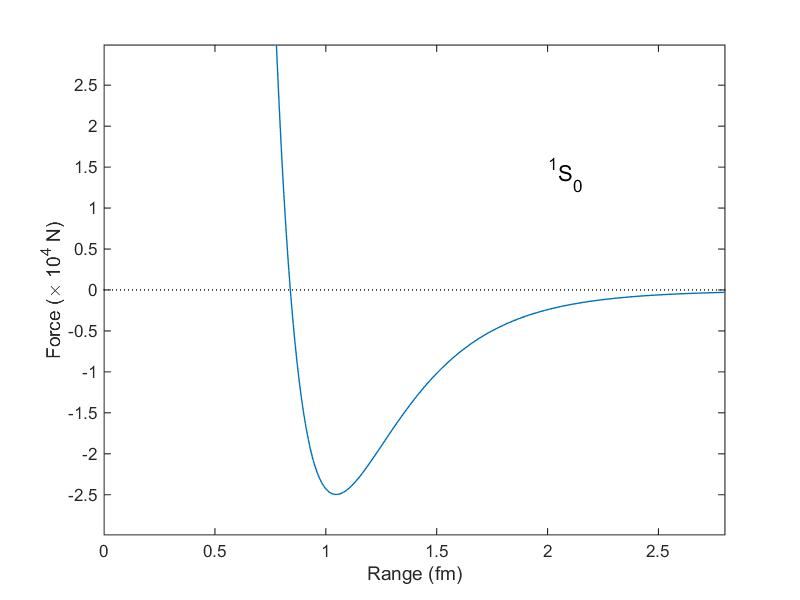
\includegraphics[width=\textwidth]{../Figures/intro_figs/ReidForce2.jpg}
	\caption{An example nucleon-nucleon potential from the Reid model~\citep{reid1968} of the nuclear force. Note the characteristic exponential decay in the attractive tail, as well as the strong repulsion that tends toward infinity at $R\approx0.7$. Figure from~\citep{bdushaw}.}
	\label{fig:reid}
\end{figure}

The specific subbranch of nuclear physics this thesis focuses on is the realm of low-energy nuclear physics.
At this level, relativistic effects are typically neglected and the nuclei are modeled as collections of protons and neutrons interacting with each other to form a bound system.
The force felt by the nucleons themselves is an artifact of the strong interaction, mediated primarily by the exchange of virtual pions with an effective range of about~$1$~fm.
Through further contributions by vector mesons (principally rho and omega), a complicated model of interacting nucleons can be built that depends on not only a nucleon's charge and distance, but also on its spin and angular momentum as well.
An example channel of the Reid potential~\citep{reid1968} is shown in Fig.~\ref{fig:reid}.
Extensive effort has been placed in modeling nuclei using such an interaction (see ~\citep{wiringa1995} for another popular choice of an N-N potential), though this \textit{ab initio} approach is not numerically feasible for large nuclei or for simulating dynamical interactions between nuclei.
It is for this reason that alternate approaches to modeling finite nuclei have been pursued throughout the field's history.

One such approach is that of the mean-field method which, simply stated, assumes that each nucleon moves freely through an average field made up of contributions from all the other nucleons.
This independent particle approximation is extremely powerful because it reduces a series of N-body self interactions to a simple sum over each individual particle.
%in the mean-field.
%A schematic image is shown in Fig.~\ref{fig:meanfield}.
While many takes on the mean-field idea have been pursued over time, the foundation of the current work was formulated in 1928 when Hartree developed the self-consistent field method~\citep{hartree1928}.
This was further extended for antisymmetric systems by Fock to form the more complete Hartree-Fock method that has been used since~\citep{fock1930}.
The term "self-consistent" used above refers to the fact that the effective Hamiltonian of the system depends on the single particle wave functions themselves, thus requiring the problem to be solved iteratively.
One common approach is to choose an initial guess of Gaussian wave packets for the first step and then a minimization procedure is followed to obtain the ground state solution for the nucleus.
Despite having a general purpose algorithm for self-consistently solving the static many-body quantum problem, the method wasn't widely adopted until computational abilities were readily available due to the large matrices involved in larger systems paired with the iterative nature of the problem.


While the Hartree-Fock method provides a general purpose, robust numerical algorithm, it is only useful for studying static properties of nuclei.
To obtain a time-dependent theory based on the mean-field approximation, one may proceed in several ways\footnote{For a more complete description of the various approaches to deriving TDHF (including a path integral formulation, many-body perturbation theory, the Balian-V\'en\'eroni variational principle, etc) see~\citep{simenel2018}.} though we will focus on the derivation by minimization of the Dirac action.
As it's vital to all chapters of this thesis and reveals much about the approximations and limitations of the theory, I will cover the derivation in detail.
First, consider the Dirac action from $t_0$ to $t_1$,
\begin{equation}
S\equiv S_{t_0,t_1}[\Psi] = \int_{t_0}^{t_1}dt \langle \Psi(t) | \left(i\hbar\frac{d}{dt}-\hat{H}\right)|\Psi(t)\rangle.
\end{equation}
For a generic many-body wave function, $|\Psi(t)\rangle$, the stationary solution of the action will simply be the Schr\"odinger equation, thus we impose that the many-body wave function is a Slater determinant of independent particle states $|\phi_i(t)\rangle$ to obtain
\begin{equation}
S_{t_0,t_1}[\Psi] = \int_{t_0}^{t_1}dt \left(\sum_{i=1}^{N} \langle\phi_i(t)|i\hbar\frac{d}{dt}|\phi_i(t)\rangle-\langle\phi_i(t)|\hat{H}|\phi_i(t)\rangle\right).
\end{equation}
This can be simplified further by defining the quantity $\sum_{i=1}^{N}\langle\phi_i(t)|\hat{H}|\phi_i(t)\rangle$ as an energy density functional (EDF), $E[\rho(t)]$.
Now, by varying with respect to single particle states we may impose the stationarity of the action
\begin{equation}
\frac{\delta S}{\delta\langle\phi_i(t)|}=i\hbar\frac{d}{dt}|\phi_i(t)\rangle - \int_{t_0}^{t_1}dt' \frac{\delta E[\rho(t)]}{\delta\langle\phi_i(t)|} = 0,
\end{equation}
with the final step being to utilize the chain rule in the EDF integral and define a final quantity, the single particle Hamiltonian, $h[\rho(t)]=\frac{\delta E[\rho(t)]}{\delta\rho(t)}$.
Collecting all of this, we are left with our final TDHF equation
\begin{equation}
i\hbar\frac{d}{dt}|\phi_i(t)\rangle = h[\rho(t)]|\phi_i(t)\rangle.
\label{eq:tdhf}
\end{equation}
By examining the form of the TDHF equations, we see that we have a description of the time evolution for each state, $i$, in the system.
Furthermore, the single particle Hamiltonian has a dependence on $\rho(t)$ and thus on the wave functions themselves.
This is in line with the self consistency feature of static Hartree-Fock mentioned above, and thus in the time propagation procedure densities from a half time step are typically used for stability.

\begin{figure}[t]
	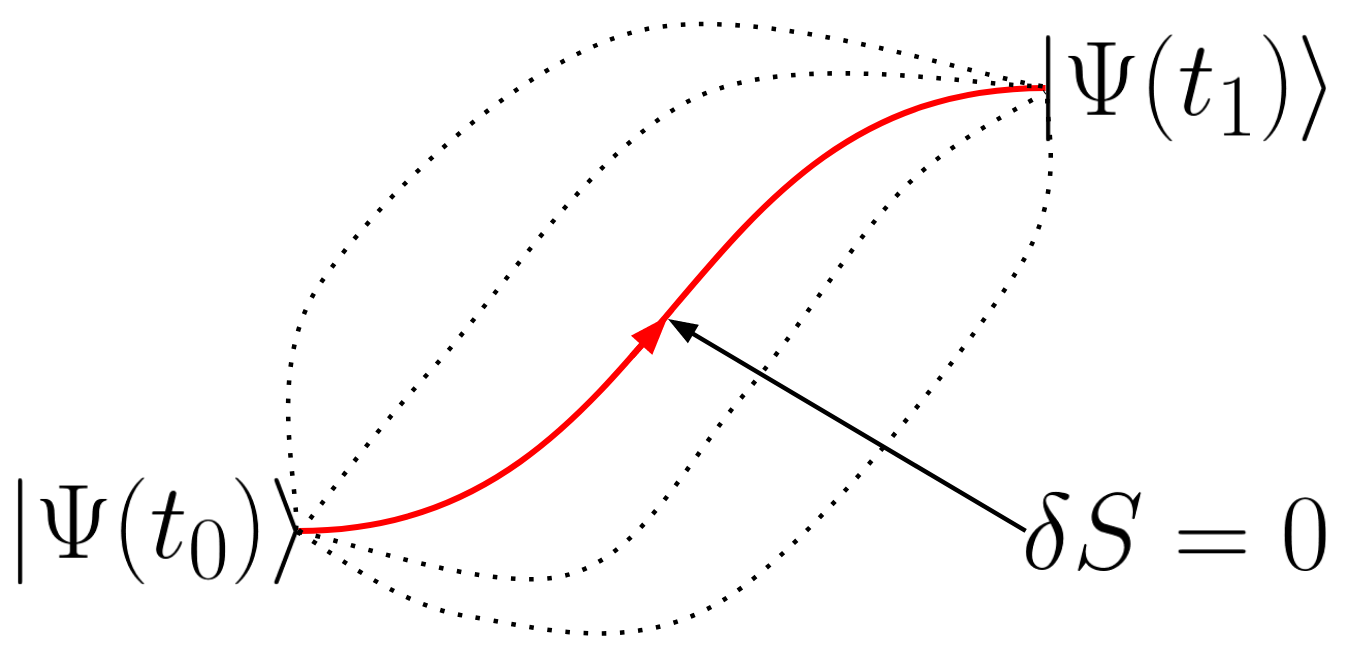
\includegraphics[width=\textwidth]{../Figures/intro_figs/paths.png}
	\caption{A schematic depiction of the stationary path chosen for the TDHF evolution.}
	\label{fig:paths}
\end{figure}

An extremely important feature of the TDHF method comes about by restricting ourselves to the stationary path from $t_0$ to $t_1$, namely that we recover only a single path in time.
This is at odds with a fully quantum picture of a many-body system evolving in time where multiple paths have some probability of occurring.
Figure~\ref{fig:paths} shows a schematic explanation of this choice.
It is for this reason that TDHF is described as a semi-classical theory and only recovers the most probable event in a time evolution.
Beyond this, the derivation required us to consider fully independent particles, just as assumed in the Hartree-Fock method, meaning that many-body correlations will not be considered.
As will be seen later in this thesis, these (and other) limitations require extensions to the base theory to uncover features in nuclear reactions that are absent with the present formulation.
Despite the theoretical shortcomings of the approach, pure TDHF calculations have been extremely successful in reproducing experimental data over its history.

One final point of interest to note from the derivation above is the appearance of a density dependent single particle Hamiltonian in Eq.~\ref{eq:tdhf}.
As this Hamiltonian was derived by varying an EDF by the density, it allows one to skip a standard representation of the interaction between nucleons as a one or two-body potential and write down the EDF directly.
This is now the standard approach in mean-field, low-energy nuclear physics and there are various forms and fits of functionals that are in active use such as Skyrme and Gogny~\citep{skyrme1956,decharge1980}.
In practice, the nuclear EDF also depends on other quantities such as the probability current, spin density, spin-current density, and so on.
The interaction used in the results presented in the current work are of the Skyrme type and the specific EDFs are noted in the individual chapters' method sections.
%This approach is justified by the Hohenberg-Kohn theorems which prov~\citep{hohenberg1964}

The specific mean-field and beyond mean-field approaches to each project presented in this work are discussed in their respective chapters, though a general, brief word should be said about the validity of the mean-field method as it applies to atomic nuclei.
As the nucleus is traditionally thought of as a densely packed collection of nucleons, the primary assumption that individual protons and neutrons can travel freely in the nucleus is a bit counter intuitive.
It turns out, however, that the Pauli exclusion principle between nucleons ensures that the particles will remain at an average distance exceeding their radius at low energies~\citep{ring1980}.
Even at finite collision energies, the mean free path of nucleons in the nucleus is several times that of the nuclear radius, implying that a so-called hard-core collision is unlikely.
This means that the average potential felt by the nucleons in the nucleus will be around the minimum of a model potential like the one shown in Fig.~\ref{fig:reid}.
Should one go to higher collision energies, the mean-field approximation begins to break down and may misrepresent the outcome of such reactions.

\section{Nuclear dynamics}

\begin{figure}[t]
	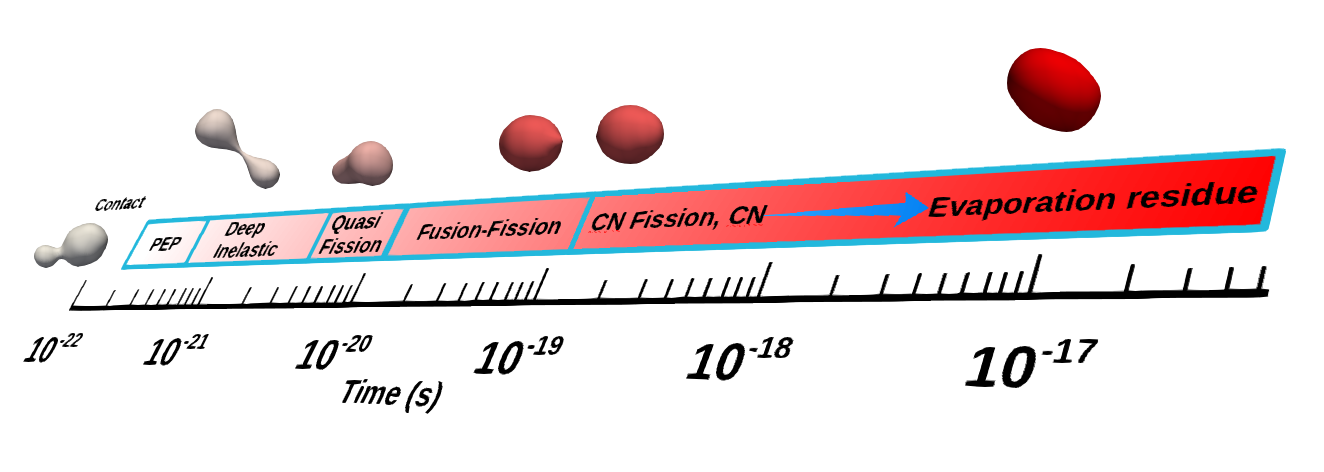
\includegraphics[width=\textwidth]{../Figures/intro_figs/timescale.png}
	\caption{The general timescales of nuclear reactions from quasielastic scattering through fusion and subsequent decay.}
	\label{fig:timescale}
\end{figure}

Our focus is now turned to the dynamics of nuclear physics at low collision energies as predicted by TDHF.
Broadly speaking, for two incoming nuclei with their own distinct numbers of protons and neutrons, one could expect to see a large number of possible outcomes depending on factors such as the orientation of the incoming nuclei, the distance off the collision axis, and the energy between the two fragments.
What is seen experimentally will be some complex combination of initial configurations, however.
The typical technique employed to investigate a given system is then to perform a large number of calculations across the configuration space in an attempt to understand what is happening systematically as you change any initial quantity.
It is for this reason that one must take care to check the full parameter space in order to make authoritative statements on the physics at play in reactions, especially when comparing to experimental data.

The usual method of classifying nuclear reactions is by the length of time that the fragments stay in contact\footnote{The specific definition of contact varies from work to work, though it is typically stated as when the density in the neck region between the nuclei is around half the saturation density, $\rho=0.08$.} before coming apart again.
Of course, if the fragments stay together indefinitely this is interpreted as a fusion event in TDHF.
Though the timescales and definition of reaction channels are fluid, they may be roughly divided into categories as is shown in Fig.~\ref{fig:timescale}.
For reasons mentioned in the previous section TDHF is capable of investigating reaction mechanisms from the far left of the chart up through compound nucleus formation (around $10^{-20}-10^{-19}$s in Fig.~\ref{fig:timescale}).
Any subsequent events after a fused system is formed, like fission or the evaporation of a particle, will not occur in a TDHF calculation and must be dealt with using a separate technique.

\begin{figure}[t]
	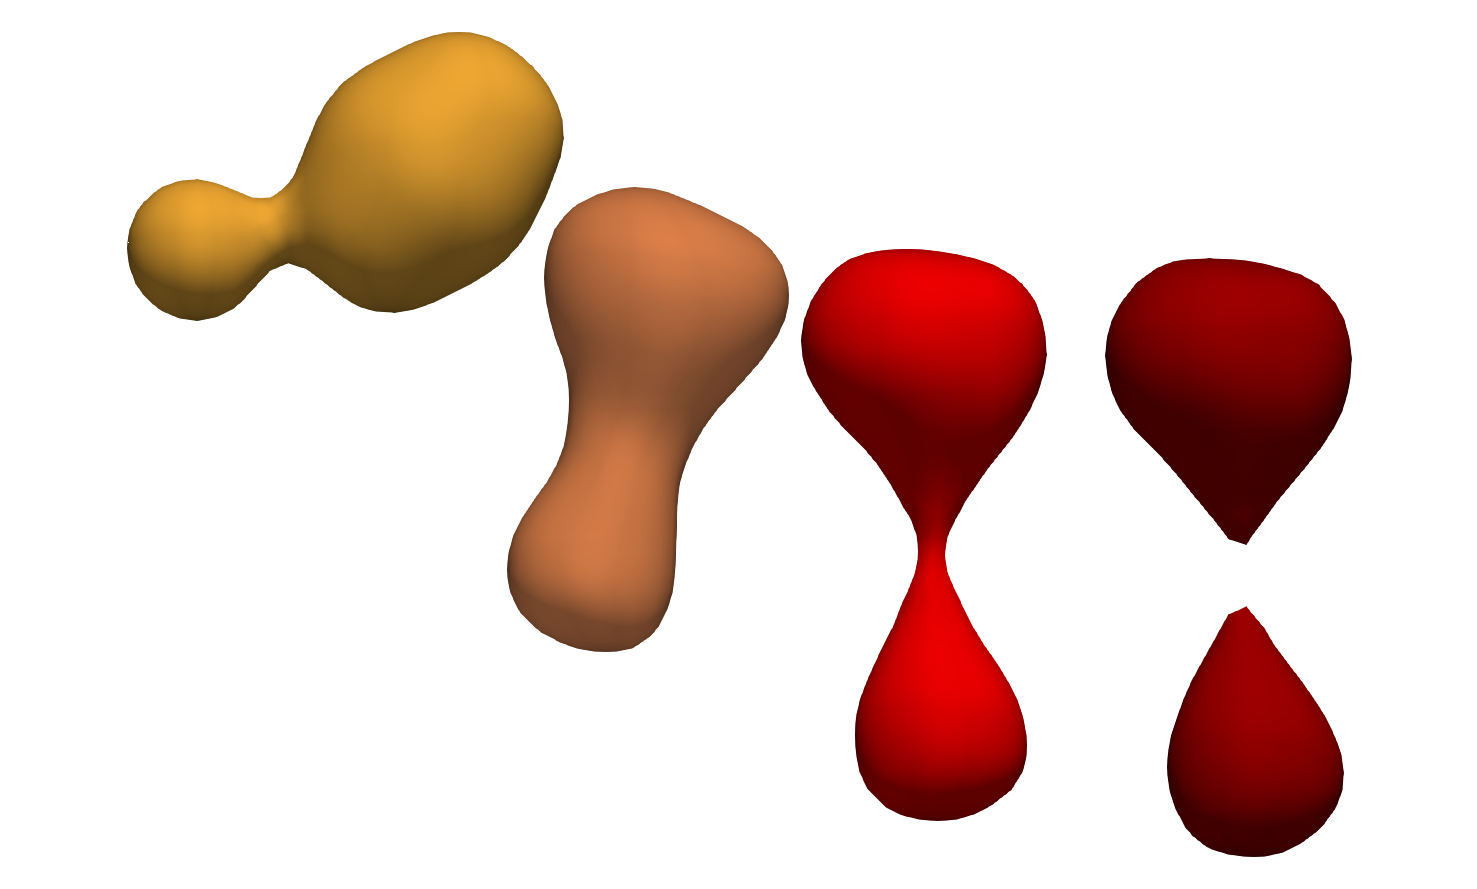
\includegraphics[width=\textwidth]{../Figures/intro_figs/48Ca249BkEvolution_tr.png}
	\caption{A typical density evolution for a quasifission reaction. The system presented is $^{48}$Ca$+^{249}$Bk and the figure is taken from~\citep{godbey2020}.}
	\label{fig:qf}
\end{figure}

As an example case, a typical set of contours from a benchmark quasifission reaction may be seen in Fig.~\ref{fig:qf}.
In this reaction, as is common in quasifission, the initially mass asymmetric system collides and begins to exchange a substantial amount of energy and mass before rotating and forming two new nuclei as they separate.
As mentioned before, the nuclei produced in such a reaction will depend on the initial configuration, and substantial effort has been expended to understand the production rates of nuclei via these sorts of reactions.
From the image it is clear that the dynamics governing the outcome of a nuclear collisions depend on much more than the incoming number of particles, hence the sophisticated tools required to study these processes.

\section{Summary}

Through use of state-of-the-art many-body methods this thesis explores nuclear reactions through both theoretical development and extensions of the base theories, as well as through systematic, comprehensive studies of nuclei.
Each chapter either focuses on a specific aspect of nuclear reactions or attempts to exhaustively characterize a given system.
In Chapter~\ref{chapters:chapter_2}, I discuss the development of a new extension to explore the role of transfer in the initial stages of the collision on fusion.
The basis of the technique is described and then select applications are presented to demonstrate the applicability to generic nuclear systems.
Chapter~\ref{chapters:chapter_3} meanwhile continues to focus on fusion, though via a more basic aspect.
Specifically, a method is developed to directly show the impact of the Pauli exclusion principle on heavy ion collisions at low energies.


Chapters~\ref{chapters:chapter_4} and~\ref{chapters:chapter_5} turn away from the development of new extensions to TDHF and instead look into the effect of the Skyrme tensor interaction on fusion for multiple systems.
Similar to this is Chapter~\ref{chapters:chapter_6} which studies fusion cross sections of \textsuperscript{12}C+\textsuperscript{12}C both above and below the fusion barrier.
This study also represents an effort to make extremely precise fusion calculations be checking the effect of numerical changes on the results.

Finally, the last two chapters are largely devoted to transfer studies for two systems of nuclei.
Chapter~\ref{chapters:chapter_7} utilizes direct TDHF collisions to study fragment production in $^{48}$Ca+$^{249}$Bk reactions.
Due to the deformed nature of $^{249}$Bk, a complete sweep of angles was performed to paint the fullest picture yet of quasifission in TDHF.
While also a study of transfer, Chapter~\ref{chapters:chapter_8} goes beyond TDHF to look at fluctuations about the mean field to uncover the correlations that are missing in the base theory.
This system, as did the one before, requires a large amount of computation due to the deformed initial states and the added cost of the beyond TDHF method.




\clearpage


%%
%% Chapter 2
% This is an example for a chapter, additional chapter can be added in the 
% skeleton-thesis.
% To generate the final document, run latex, build and quick build commands
% on the skeleton-thesis file not this one.

\makeatletter
\renewcommand{\AB@affillist}{}
\renewcommand{\AB@authlist}{}
\setcounter{authors}{0}
\setcounter{affil}{0}
\makeatother

\chapter{Dependence of fusion on isospin dynamics}\label{chapters:chapter_2}
%\vspace{-7mm}

{
\title{Dependence of fusion on isospin dynamics}

\author[1]{K. Godbey}
\author[1]{A.S. Umar}
\affil[1]{Department of Physics and Astronomy, Vanderbilt University, Nashville, TN 37235}

\author[2]{C. Simenel}
\affil[2]{Department of Nuclear Physics, Research School of Physics and Engineering, The Australian National University, Canberra ACT  2601, Australia}


	\bfseries\centering
	The following work has been accepted by Physical Review C~\citep{godbey2017} and is reprinted below in its entirety.\\
	\textcopyright2017 American Physical Society
	\makeatletter
	\begin{center}\large\bfseries
		\@title
		\par\end{center}
	\begin{center}
		\AB@authlist
		
		\AB@affillist
	\end{center}
	\makeatother
}
\makeatletter
\renewcommand{\AB@affillist}{}
\renewcommand{\AB@authlist}{}
\setcounter{authors}{0}
\makeatother





\section*{Abstract}
	We introduce a new microscopic approach to calculate the dependence of fusion barriers and cross-sections on
	isospin dynamics. The method is based on the time-dependent Hartree-Fock theory and
	the isoscalar and isovector properties of the energy density functional (EDF). The contribution to
	the fusion barriers originating from the isoscalar and isovector parts of the EDF is calculated.
	It is shown that for non-symmetric systems the isovector dynamics influence the sub-barrier fusion
	cross-sections. For most systems this results in an enhancement of the sub-barrier cross-sections,
	while for others we observe differing degrees of hindrance.
	We use this approach to provide an explanation of recently measured fusion cross sections which show a  enhancement at low $E_\mathrm{c.m.}$ energies
	for the system $^{40}$Ca+$^{132}$Sn as compared to the more neutron-rich system
	$^{48}$Ca+$^{132}$Sn, and discuss the dependence of sub-barrier fusion cross-sections on transfer.
	
\section{Introduction}

One of the major open questions in fusion reactions of exotic neutron-rich nuclei
is the dependence of the fusion cross section on the neutron excess,
or equivalently on the total isospin quantum number $T_z = (Z-N)/2$.
This is a timely subject given the expected
availability of increasingly exotic beams at rare isotope facilities\,\citep{balantekin2014}.
The influence of isospin dynamics on fusion is also one of the key questions pertaining to the
production of superheavy elements using neutron rich nuclei\,\citep{loveland2007}.
Besides being a fundamental nuclear structure and reaction question, the answer to this inquiry
is also vital to our understanding of the nuclear equation of state (EOS) and symmetry energy\,\citep{li2014}.
The EOS plays a key role in elucidating the structure of exotic nuclei\,\citep{chen2015},
the dynamics of heavy ion collisions\,\citep{danielewicz2002,tsang2009},
the composition of neutron stars\,\citep{haensel1990,chamel2008,horowitz2004,utama2016}, and the mechanism of core-collapse supernovae\,\citep{bonche1981,watanabe2009,shen2011}.
The influence of isospin flow during heavy-ion reaction is usually discussed in term of the
$(N/Z)$ asymmetry of the target and projectile or the $Q$-values for nucleon transfer.

The presence of positive $Q-$value transfer channels has been shown to enhance sub-barrier fusion in various systems~\citep{jiang2014a}.
However, what affects the magnitude of this enhancement is still actively debated~\citep{kohley2011,kohley2013,kolata2012,jiang2015,liang2016}.
In particular, recent experiments carried out
with radioactive $^{132}$Sn beams and with stable $^{124}$Sn beams on
$^{40,48}$Ca~\citep{kolata2012} and $^{58,64}$Ni~\citep{kohley2011} targets have shown that the enhancement is observed at much lower cross-sections in the heavier (Ni+Sn) systems~\citep{jiang2015} than in the lighter (Ca+Sn) ones.
Various possible effects have been invoked to explain these observations~\citep{liang2016},
such as a larger role of dissipation due to the increase of the charge product $Z_1Z_2$ of the collision partners~\citep{wolfs1987,evers2011,rafferty2016}.
%J'en suis la
It is also known that for systems with $Z_1Z_2\gtrsim1600$, the so-called quasifission, where the nuclei re-separate after a significant mass transfer, strongly hinders fusion~\citep{toke1985}.

The effect of neutron transfer on fusion is traditionally described  within the coupled-channels (CC) method~\citep{rowley1992,esbensen1998,hagino2012}
and models incorporating intermediate neutron
rearrangements\,\citep{zagrebaev2003,zagrebaev2007c,karpov2015}.
These approaches, however, model the transfer process on a schematic way
and they require nuclear data which are often unknown for exotic nuclei.
New approaches are then needed to describe realistically the effect of both proton and neutron transfers on fusion of stable and exotic nuclei.
In particular, dissipation induced by transfer should be properly accounted for.

Here, we take a first step toward this ambitious theoretical program by investigating the overall effect of isospin dynamics induced mostly by neutron and/or proton transfer in collisions of asymmetric systems~\citep{dasso1985,chomaz1993,baran1996,baran2001,simenel2001,baran2005,simenel2007,baran2009,oberacker2012,umar2008a}.
In particular, we address the impact of isospin dynamics on fusion barriers and cross-sections using
the microscopic
time-dependent Hartree-Fock (TDHF) theory\,\citep{negele1982,simenel2012}
together with the density-constrained TDHF (DC-TDHF) method for calculating fusion barriers\,\citep{umar2006b}.
This choice is motivated by the fact that the TDHF approach has been used to successfully describe multinucleon transfer~\citep{simenel2010,simenel2012b,sekizawa2013,scamps2013a,bourgin2016}, as well as strongly damped reactions such as deep-inelastic collisions~\citep{koonin1977,simenel2011} and quasi-fission~\citep{wakhle2014,umar2015a,umar2016}, without relying on an {\it a priori} knowledge of the structure of the reactants.
Therefore, these microscopic dynamical calculations incorporate the fundamental mechanisms which are relevant for a realistic description of the effect of transfer on fusion, including with exotic beams.
As a first application, various systems from Ca+Ca to Ca+Sn are considered.

\section{Formalism}

In the TDHF approximation the many-body wavefunction is replaced by a single
Slater determinant and this form is preserved at all times, implying that two-body correlations
are neglected.
In this limit, the
variation of the time-dependent action with respect to the single-particle states, $\phi^{*}_{\lambda}$, yields the most probable time-dependent path
in the multi-dimensional space-time phase space
represented as a
set of coupled, nonlinear, self-consistent initial value equations
for the single-particle states
\begin{equation}
h(\{\phi_{\mu}\}) \ \phi_{\lambda} (r,t) = i \hbar \frac{\partial}{\partial t} \phi_{\lambda} (r,t)
\ \ \ \ (\lambda = 1,...,A)\,,
\end{equation}
where $h$ is the HF single-particle Hamiltonian.
These are the fully microscopic time-dependent Hartree-Fock equations.

Almost all TDHF calculations employ the Skyrme EDF, which allows the total energy of the system to be represented
as an integral of the energy density ${\cal H}(\mathbf{r})$\,\citep{engel1975}
\begin{equation}
\label{eq:energy}
E = \int d^3\mathbf{r} {\cal H}(\mathbf{r})\,,
\end{equation}
which includes the kinetic,
isoscalar, isovector, and Coulomb terms \,\citep{dobaczewski1995}:
\begin{equation}
\label{eq:edensity}
{\cal H}(\mathbf{r}) = \frac{\hbar^2}{2m}\tau_0
+ {\cal H}_0(\mathbf{r})
+ {\cal H}_1(\mathbf{r})
+ {\cal H}_C(\mathbf{r})\,.
\end{equation}
In particular,
	\begin{equation}
	\label{eq:efunctional}
	{\cal H}_\mathrm{I}(\mathbf{r})
	= C_\mathrm{I}^{\rho}            \rho_\mathrm{I}^2
	+  C_\mathrm{I}^{   s}            \mathbf{s}_\mathrm{I}^2
	+  C_\mathrm{I}^{\Delta\rho}      \rho_\mathrm{I}\Delta\rho_\mathrm{I}
	+  C_\mathrm{I}^{\Delta s}        \mathbf{s}_\mathrm{I}\cdot\Delta\mathbf{s}_\mathrm{I}
	+  C_\mathrm{I}^{\tau}      \left(\rho_\mathrm{I}\tau_\mathrm{I}-\mathbf{j}_\mathrm{I}^2  \right)
	+  C_\mathrm{I}^{   T}      \Big(\mathbf{s}_\mathrm{I}\cdot
	\mathbf{T}_\mathrm{I} - \tensor{J}_\mathrm{I}^2\Big)
	+ C_\mathrm{I}^{\nabla J}  \Big(\rho_\mathrm{I}\mathbf{\nabla}\cdot\mathbf{J}_\mathrm{I}
	+ \mathbf{s}_\mathrm{I}\cdot
	(\mathbf{\nabla}\times\mathbf{j}_\mathrm{I})\Big)\,,
	\end{equation}

where we have used the gauge invariant form suitable for time-dependent calculations.
The isospin index $\mathrm{I}=0,1$ for isoscalar and isovector energy densities, respectively.
The most common choice of Skyrme EDF restricts the density dependence of the
coupling constants to the $C_\mathrm{I}^{\rho}$ and $C_\mathrm{I}^s$ terms only.
These density dependent coefficients contribute to the coupling of isoscalar and isovector fields
in the Hartree-Fock Hamiltonian.
The isoscalar (isovector) energy density, ${\cal H}_0(\mathbf{r})$ (${\cal H}_1(\mathbf{r})$), depends on the isoscalar (isovector) particle
density, $\rho_0 = \rho_n + \rho_p$ ($\rho_1 = \rho_n - \rho_p$), with analogous expressions for other densities and
currents.
Values of the coupling
coefficients as well as their relation to the alternative parametrizations of the Skyrme
EDF can be found in\,\citep{dobaczewski1995}.
\begin{figure}
	\includegraphics*[width=\textwidth]{../Figures/Isospin/V_40_48Ca.pdf}
	\caption{For the $^{40}$Ca+$^{48}$Ca system;
		Total and isoscalar DC-TDHF potentials. The shaded region
		corresponds to the reduction originating from the isovector contribution to the energy
		density. The insert shows the isoscalar and isovector contributions to the interaction barrier
		without the Coulomb potential.
		The TDHF collision energy was $E_\mathrm{c.m.}=55$\,MeV.}
	\label{fig:CaCa}
\end{figure}

The above form of the EDF is more suitable for studying the isospin dependence
of nuclear properties and have been employed in nuclear structure studies\,\citep{dobaczewski1995}.
In the same spirit we can utilize this approach to study isospin dependent effects in nuclear
reactions microscopically.
In particular, the density-constrained time-dependent Hartree-Fock (DC-TDHF) method\,\citep{umar2006b} can be
employed to study isospin effects on fusion barriers and fusion cross-sections.
The DC-TDHF approach calculates the nucleus-nucleus potentials $V(R)$ directly
from  TDHF dynamics and has been used to calculate fusion cross-sections for a wide range of
reactions\,\citep{umar2014a,simenel2013a,umar2012a,umar2006a,oberacker2010,umar2009a,jiang2015a}.
The basic idea of this approach is the following:
At certain times $t$ or, equivalently, at certain internuclear distances
$R(t)$, a static energy minimization
is performed while constraining the proton and neutron densities to be equal to the instantaneous
TDHF densities.
We refer to the minimized energy as the ``density constrained energy''
$E_{\mathrm{DC}}(R)$.
The ion-ion interaction potential $V(R)$ is obtained by
subtracting the constant binding energies
$E_{\mathrm{A_{1}}}$ and $E_{\mathrm{A_{2}}}$ of the two individual nuclei
\begin{equation}
V(R)=E_{\mathrm{DC}}(R)-E_{\mathrm{A_{1}}}-E_{\mathrm{A_{2}}}\ .
\label{eq:vr}
\end{equation}
The calculated ion-ion interaction barriers contain all of the dynamical changes in the nuclear
density during the TDHF time-evolution in a self-consistent manner.
As a consequence of the dynamics the DC-TDHF potential is energy dependent\,\citep{umar2014a}.
Using the decomposition of the Skyrme EDF into isoscalar and isovector parts [Eq.\,(\ref{eq:efunctional})],
we can re-write this potential as
\begin{equation}
V(R) = \sum_{\mathrm{I}=0,1} v_\mathrm{I}(R) + V_C(R)\,,
\end{equation}
where $v_\mathrm{I}(R)$ denotes the potential computed by using the isoscalar and isovector parts of
the Skyrme EDF given in Eq.\,(\ref{eq:edensity}) in Eq.\,(\ref{eq:vr}).
The Coulomb potential is also calculated via Eq.\,(\ref{eq:vr}) using the Coulomb energy
density.
\begin{figure}
	\includegraphics*[width=\textwidth]{../Figures/Isospin/V_16O_208Pb_ecm75.pdf}
	\caption{For the $^{16}$O+$^{208}$Pb system;
		(a) Total and isoscalar DC-TDHF potentials at $E_\mathrm{c.m.}=75$\,MeV. The shaded
		region corresponds to the reduction originating from the isovector contribution to
		the energy density.
		(b) Same as in (a) except for $E_\mathrm{c.m.}=90$\,MeV.
		(c) Same as in (a) except for $E_\mathrm{c.m.}=120$\,MeV.}
	\label{fig:OPb}
\end{figure}
\begin{figure}
	\includegraphics*[width=\textwidth]{../Figures/Isospin/V_CaTi_Pb_stack_2.pdf}
	\caption{Isoscalar and isovector breakdown of the potential barrier for two
		systems at the same $E_\mathrm{c.m.}/V_B=1.065$;
		(a) $^{48}$Ca+$^{208}$Pb. The shaded region corresponds to the increase originating
		from the isovector contribution to
		the energy density.
		(b) Same as in (a) except $^{50}$Ti+$^{208}$Pb.
		The shaded region corresponds to the decrease originating from the isovector contribution to
		the energy density.}
	\label{fig:CaTi_Pb}
\end{figure}

\section{Results}

We have used the DC-TDHF approach to study fusion barriers for a number of systems.
Calculations were done in a three-dimensional
Cartesian geometry with no symmetry assumptions\,\citep{umar2006c} and using the
Skyrme SLy4 EDF\,\citep{chabanat1998a}.
The three-dimensional Poisson equation for the Coulomb potential
is solved by using Fast-Fourier Transform techniques
and the Slater approximation is used for the Coulomb exchange term.
The box size used for all the calculations
was chosen to be $60\times 30\times 30$~fm$^3$, with a mesh spacing of
$1.0$~fm in all directions. These values provide very accurate
results due to the employment of sophisticated discretization
techniques\,\citep{umar1991a}.
\begin{figure}
	\includegraphics*[width=\textwidth]{../Figures/Isospin/V_Ca_Sn_stack.pdf}
	\caption{For     (a) $^{40}$Ca+$^{132}$Sn,
		(b) $^{48}$Ca+$^{132}$Sn
		%(c) $^{54}$Ca+$^{132}$Sn
		systems;
		Total and isoscalar DC-TDHF potentials. In (a) the blue shaded region
		corresponds to the reduction originating from the isovector contribution.
		In (b) we see no isovector effect. (c) the isovector effect is reversed
		causing hindrance as shown by the red shaded region.
		The inserts show the isoscalar and isovector contributions to the interaction barrier without the Coulomb potential.
		The TDHF collision energy was $E_\mathrm{c.m.}=120$\,MeV.}
	\label{fig:CaSn_1}
\end{figure}
%\onecolumngrid
\begin{figure}
	\centering
	\includegraphics*[width=\textwidth]{../Figures/Isospin/current.pdf}
	\caption{Neutron and proton current vectors in $^{40,48}$Ca+$^{132}$Sn at $E_\mathrm{c.m.}=120$\,MeV and at
		a separation  $R=11.5$\,fm between the fragments.}
	\label{fig:current}
\end{figure}
%\twocolumngrid

In Fig.\,\ref{fig:CaCa} we show the total and isoscalar fusion barriers (both including the Coulomb contribution)
for the $^{40}$Ca+$^{48}$Ca system at $E_\mathrm{c.m.}=55$~MeV.
For the Ca+Ca systems the energy dependence is relatively
weak\,\citep{keser2012,umar2014a,washiyama2008}.
The reduction of the isoscalar barrier is due to the isovector contribution. It is evident that
the isovector dynamics results in the narrowing of the fusion barrier, thus resulting in an enhancement of the sub-barrier
fusion cross-sections. The insert in Fig.\,\ref{fig:CaCa} shows the isovector and isoscalar components without the Coulomb contribution.
We have also calculated fusion barriers for the $^{40}$Ca+$^{40}$Ca and $^{48}$Ca+$^{48}$Ca systems, where the isovector contribution is
zero as expected from symmetry.
Irrespective of its isovector/isoscalar nature, the DC-TDHF potential is a way to represent the potential felt by the system at a given time. The relation between time and distance between the fragments then allow to represent the potential in the traditional manner, i.e., as a function of the internuclear distance. The fact that the isovector reduction occurs essentially inside the barrier indicates that the proton and neutron flows become larger for stronger overlap occurring in the later stage of fusion.

As an example of a more asymmetric system we performed calculations for the $^{16}$O+$^{208}$Pb system
at $E_{\mathrm{c.m.}}=75$\,MeV. Results are shown in Fig.\,\ref{fig:OPb}(a). Here we see a
substantial enhancement of sub-barrier fusion due to the isovector dynamics.
For this system we have performed further
calculations at c.m. energies of 90\,MeV and 120\,MeV shown in Fig.\,\ref{fig:OPb}(b-c).
As the beam energy  increases, the
relative contribution from the isovector component to the total barrier decreases, while the overall barrier height increases with
increasing energy. At TDHF energies much higher than the barrier height the total barriers approaches the frozen density
barrier\,\citep{washiyama2008,umar2014a}
due to the inability of the system to rearrange at that time-scale at which time the isovector contribution vanishes as well.
Next, we have calculated isoscalar and isovector breakdown of the potential barrier for two
systems at the same $E_\mathrm{c.m.}/V_B=1.065$ as shown in Fig.\,\ref{fig:CaTi_Pb}(a,b) for;
$^{48}$Ca+$^{208}$Pb system where the shaded region corresponds to the increase in the barrier
originating
from the isovector contribution to the energy density, and for the
$^{50}$Ti+$^{208}$Pb system where
the shaded region corresponds to the decrease in the barrier originating from the isovector
contribution to
the energy density.
The above results demonstrate the influence of isovector dynamics on typical fusion barriers.

We next look at Ca$+$Sn reactions.
The experimental observation of a sub-barrier fusion enhancement in the system $^{40}$Ca+$^{132}$Sn
as compared to more neutron-rich system $^{48}$Ca+$^{132}$Sn was the subject of a previous DC-TDHF study\,\citep{oberacker2013},
where it was shown that the fusion barriers for the two systems have essentially the same height but the fusion barrier for
the $^{48}$Ca+$^{132}$Sn system was much wider than that for the $^{40}$Ca+$^{132}$Sn system.
We see in Fig.\,\ref{fig:CaSn_1}(a) a strong reduction of the isoscalar barrier due to the isovector contribution. This behavior is similar to that of the previous
two systems albeit the isovector reduction is somewhat larger as shown in the insert of
Fig.\,\ref{fig:CaSn_1}(a).
We then performed the same calculation for the $^{48}$Ca+$^{132}$Sn system as shown in Fig.\,\ref{fig:CaSn_1}(b).
The startling result is the vanishing of the isovector contribution. With no isovector reduction the fusion barrier for this
system is much wider than that for the $^{40}$Ca+$^{132}$Sn system for which substantial reduction occurs.
The absence of the isovector component for the $^{48}$Ca+$^{132}$Sn system could be a reflection of the negative $Q-$values
for neutron pickup. This is the first direct observation of this phenomena in microscopic calculations.

This may also explain why for the $^{48}$Ca+$^{132}$Sn system simply considering the $2^+$ and
$3^-$ excitations of the target and projectile in coupled-channel calculations is able to
reproduce the sub-barrier fusion cross-sections, whereas doing the same for the $^{40}$Ca+$^{132}$Sn system grossly under-predicts the cross-sections.
In Ref.\,\citep{kolata2012}, this was attributed to transfer
%the presence of significant transfer,
which manifests itself in the isovector dynamics.
In Fig.\,\ref{fig:CaSn_1}(c) we have also calculated the potential barriers for the theoretical
$^{54}$Ca+$^{132}$Sn reaction. Here, we see that the influence of the isovector component
is reversed, as indicated by the shaded region. This reversal leads to the widening of
the potential barrier, further hindering sub-barrier fusion.

In all the studied systems, we observe an isovector reduction in the presence of  positive $Q-$values for transfer channels.
This can be understood from the $C_\mathrm{I}^{\rho}            \rho_\mathrm{I}^2$ term in Eq.~(\ref{eq:edensity})
which quantitatively dominates.
When an isospin equilibration occurs (driven by positive $Q-$values),
the $I=1$ contribution gets reduced as $(\rho_p-\rho_n)^2$ decreases
in each fragment and $C_1^\rho$ is positive.
This also explains why, in systems with only negative Q-values, the isovector contribution to the potential
vanishes.
In very few cases, such as for the theoretical $^{54}$Ca+$^{132}$Sn reaction,
we even found an increase of the
potential which is attributed to more complex density dependencies of $H_1$ in Eq.~(\ref{eq:edensity}).

In order to investigate the role of transfer in more detail we have plotted  in Fig.\,\ref{fig:current}
the microscopic TDHF neutron and proton currents for $^{40,48}$Ca$+^{132}$Sn
at  $E_\mathrm{c.m.}=120$\,MeV and  at the nuclear separation $R=11.5$\,fm,
which is slightly inside the barrier but still corresponds to an early stage of the reaction.
%for the same collision energy used to calculate the barriers shown in Fig.\,\ref{fig:CaSn_1}
In $^{40}$Ca+$^{132}$Sn, neutrons flow from Sn to Ca (Fig.~\ref{fig:current}a) and protons from Ca to Sn (Fig.~\ref{fig:current}c),
compatible with the fact that there are many positive $Q-$value channels for these transfers to occur.
For $^{48}$Ca$+^{132}$Sn, which has no positive $Q-$value transfer channel,
we observe a convergence of neutrons towards the neck (Fig.~\ref{fig:current}b),
which is what we would expect in the fusion process.
This is also what is observed for protons in (Fig.~\ref{fig:current}d),
although there is a larger displacement of protons from Ca towards the
neutron-rich neck. %Nevertheless, this does not correspond to a transfer
%of protons as the proton flow in the tin is also directed towards the neck,
%which is compatible with the fact that there is no positive $Q-$value for
%proton transfer in this system.
%Examination of these currents shows that for
%the $^{40}$Ca+$^{132}$Sn system neutrons flow from $^{132}$Sn to
%$^{40}$Ca, whereas the proton flow is from $^{40}$Ca to $^{132}$Sn.
%Proton flow for the $^{48}$Ca+$^{132}$Sn system is similar, namely from $^{48}$Ca to
%$^{132}$Sn. However, we observe an interesting difference for the neutron flow in the
%$^{48}$Ca+$^{132}$Sn system, namely a bi-directional flow between the two systems.
%The dynamics of this bi-directional flow results in
As a result, the isovector current density in the neck region is an order of magnitude lower
for the $^{48}$Ca+$^{132}$Sn system in comparison to the $^{40}$Ca+$^{132}$Sn.
\begin{figure}
	\centering
	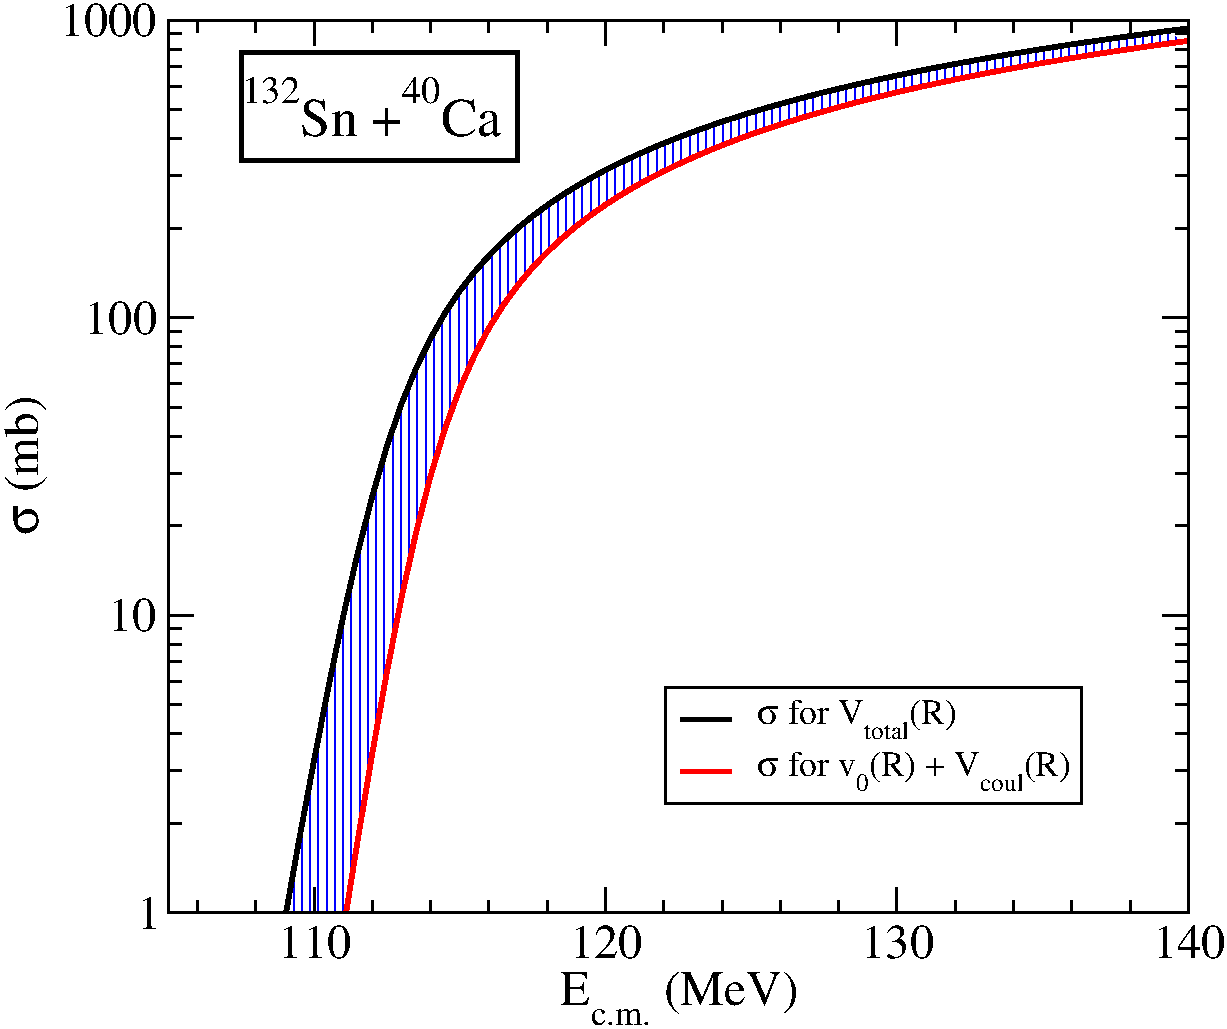
\includegraphics[width=\textwidth]{../Figures/Isospin/x_40Ca_132Sn.pdf}
	\caption{Fusion cross-section  in $^{40}$Ca+$^{132}$Sn calculated with (black line) and without (red line) isovector reduction, using the potentials of Fig.~\ref{fig:CaSn_1}a.}
	\label{fig:cs}
\end{figure}
This is the primary cause for the disappearance of the isovector contribution to the barrier.
%In the neck region, the relative magnitude of the proton current density of $^{48}$Ca+$^{132}$Sn system
%is 30\%-50\% smaller than the proton current density of the $^{40}$Ca+$^{132}$Sn.
%This behavior is prevalent during the entire neck dynamics.
%Examination of the currents for the $^{54}$Ca+$^{132}$Sn reaction reveals that there is
%essentially no through-flow of neutrons or protons during the neck formation.

Finally, the impact of the isovector contribution to the fusion dynamics is shown in Fig.~\ref{fig:cs},
where fusion cross-sections have been computed from the DC-TDHF potentials of Fig.~\ref{fig:CaSn_1}a.
The effect of the isovector reduction is particularly visible at sub-barrier energies where an enhancement
of the fusion cross-sections by about an order of magnitude is observed.
To our knowledge, this is the first microscopic evidence of the enhancement
of fusion due to coupling to transfer channels.

\section{Conclusion}

In summary, we have developed a microscopic approach to study the effect of isospin dynamics on fusion barriers.
We have shown that for most systems isovector dynamics results in the thinning of the barrier thus enhancing
the sub-barrier fusion cross-sections. The isovector reduction effect vanishes for symmetric systems as well
as the $^{48}$Ca+$^{132}$Sn system for which neutron pickup $Q-$values are all negative.
These results provide a quantitative measure for the importance of transfer for
sub-barrier fusion reactions.
Furthermore, they elucidate the non-trivial dependence of sub-barrier fusion for neutron-rich
systems and illustrate the importance of dynamical microscopic models that incorporate the nuclear
structure and reactions on the same footing.
%A more detailed study including cross-section ratios and other systems will be the subject of a future study.

We thank K. Vo-Phuoc for useful discussions regarding the Ca+Sn systems.
This work has been supported by the U.S. Department of Energy under grant No.
DE-SC0013847 with Vanderbilt University and by the
Australian Research Council Grant No. FT120100760.

\clearpage



%%
%% Chapter 3
% This is an example for a chapter, additional chapter can be added in the 
% skeleton-thesis.
% To generate the final document, run latex, build and quick build commands
% on the skeleton-thesis file not this one.

\chapter{How the Pauli exclusion principle affects fusion of atomic nuclei}\label{chapters:chapter_3}
\vspace{-7mm}

\author{C. Simenel}
\affil{Department of Nuclear Physics, Research School of Physics and Engineering, 
	The Australian National University, Canberra ACT  2601, Australia}

\author{A.S. Umar}
\affil{Department of Physics and Astronomy, Vanderbilt University, Nashville, TN 37235, USA}

\author{K. Godbey}
\affil{Department of Physics and Astronomy, Vanderbilt University, Nashville, TN 37235, USA}

\author{M. Dasgupta}
\affil{Department of Nuclear Physics, Research School of Physics and Engineering, 
	The Australian National University, Canberra ACT  2601, Australia}

\author{D. J. Hinde}
\affil{Department of Nuclear Physics, Research School of Physics and Engineering, The Australian National University, Canberra ACT  2601, Australia}


\section*{Abstract}
	The Pauli exclusion principle induces a repulsion between composite systems 
	of identical fermions such as colliding atomic nuclei.
	Our goal is to study how heavy-ion fusion is impacted by this ``Pauli repulsion''.
	We propose a new microscopic approach, the density-constrained frozen Hartree-Fock method, 
	to compute the bare potential including the Pauli exclusion principle exactly.
	Pauli repulsion is shown to be important inside the barrier radius and increases 
	with the charge product of the nuclei. 
	Its main effect is to reduce tunnelling probability. 
	Pauli repulsion is part of the solution to the long-standing deep sub-barrier fusion hindrance problem.

\section{Introduction}

The idea that identical fermions cannot occupy the same quantum state was proposed by 
Stoner\,\citep{stoner1924} and  generalized by Pauli\,\citep{pauli1925}. Known as the Pauli exclusion 
principle, it was at first empirical, but is now  explained by the spin-statistic theorem in quantum 
field theory\,\citep{fierz1939,pauli1940}. The importance of the ``Pauli exclusion principle'' cannot 
be overstated. For instance, it is largely responsible for the stability of matter against collapse, 
as demonstrated by the existence of white dwarfs. It is also expected to play a crucial role 
in the dynamics of  systems of identical fermions. 
For instance, it could   impact quantum tunnelling of complex systems which remains 
one of the greatest challenges of the quantum many-body problem. 
This work addresses the question of the effect of the Pauli exclusion principle on tunnelling 
of complex systems in the specific framework of nuclear physics which offers an ideal ground 
to test concepts of the quantum many-body problem.

The Pauli exclusion principle generates a repulsion between composite systems 
of identical fermions at short distance.
For example, it repels atomic electron clouds in ionic molecules due to the fermionic nature of the electron.
Another example is the hard-core repulsion between two nucleons induced 
by identical quarks of the same color present in both nucleons.
Naturally, a similar effect is expected to occur between atomic nuclei which are composite systems of nucleons.
Indeed, it has been predicted that the Pauli exclusion principle should induce a repulsion 
(called ``Pauli repulsion'' hereafter) between strongly overlapping nuclei\,\citep{fliessbach1971}.

The Pauli repulsion should then be included in the nucleus-nucleus potentials used
to model reactions such as (in)elastic scattering, (multi)nucleon transfer, and fusion.
However, Pauli repulsion is usually neglected in these models:
it has been argued that the outcome of a collision between nuclei is mostly determined
at a  distance where the nuclei do not overlap much 
and thus the effects of the Pauli exclusion principle are minimized.
This argument is based on the assumption that nuclei do not necessarily probe
the inner part of the fusion barrier.
However, at energies well above the barrier, the system could reach more compact shapes
where one cannot neglect the effect of the Pauli principle anymore,
as was shown by several authors in the 1970's\,\citep{fliessbach1971,brink1975,zint1975,beck1978,sinha1979}.
Similarly, for deep sub-barrier energies the inner turning-point of the fusion barrier entails significant overlap
between the two nuclei\,\citep{dasso2003,umar2012a}.

Using a realistic microscopic approach to compute nucleus-nucleus bare potentials,
we  show that, in fact, the Pauli repulsion plays an important role on fusion at deep sub-barrier energies.
In particular, it provides a natural (though only partial) explanation 
for the experimentally observed deep sub-barrier fusion hindrance
\citep{jiang2002,dasgupta2007,stefanini2010}   (see Ref. \,\citep{back2014} for a review)
which has led to various theoretical interpretations
\citep{misicu2006,misicu2007,dasgupta2007,diaz-torres2008,diaz-torres2010,ichikawa2009b,ichikawa2015},
although none of them directly consider Pauli repulsion as a possible mechanism.

\section{Formalism}

In order to investigate the effect of Pauli repulsion on heavy-ion fusion,
we introduce a novel microscopic method called density-constrained frozen Hartree-Fock (DCFHF)
to compute the interaction between nuclei while accounting exactly 
for the Pauli exclusion principle between nucleons.
The microscopically derived bare nucleus-nucleus potential 
including Pauli repulsion is then used to study deep sub-barrier fusion.
For simplicity, we focus on systems with doubly-magic nuclei which are spherical and non-superfluid. 
As an example, $^{16}$O$+^{16}$O, $^{40,48}$Ca$+^{40,48}$Ca, $^{16}$O,$^{48}$Ca$+^{208}$Pb
reactions are studied theoretically and compared with experimental data.

To avoid the introduction of new parameters, we adopt the idea of Brueckner \textit{et al.}\,\citep{brueckner1968}
to derive the bare potential from an energy density functional (EDF)  $E[\rho]$
written as an integral of an energy density $\mH[\rho(\vr)]$, i.e.,
\oeq
E[\rho]=\int \d\vr \sdf \mH[\rho(\vr)]\,.
\ceq
The bare potential is obtained by requiring frozen ground-state densities $\rho_{i}$ 
of each nucleus ($i=1,2$) which we compute
using the Hartree-Fock (HF) mean-field approximation\,\citep{hartree1928,fock1930}. 
The Skyrme EDF\,\citep{skyrme1956} is used both in HF calculations and to compute the bare potential.
It accounts for the bulk properties of nuclear matter such as its incompressibility
which is crucial at short distances\,\citep{brueckner1968,misicu2006,hossain2015}.
Neglecting the Pauli exclusion principle between nucleons in different nuclei
leads to the usual frozen Hartree-Fock (FHF) 
potential\,\citep{denisov2002,washiyama2008,simenel2008,simenel2012}
\oeq
V_{FHF}(\vR)=\int \d\vr \sdf \mH[\rho_1(\vr)+\rho_2(\vr-\vR)] - E[\rho_1] -E[\rho_2],
\label{eq:frozen}
\ceq
where $\vR$ is the distance vector between the centres of mass of the nuclei.
The FHF potential, assumed to be central, can then directly be used to compute
fusion cross-sections\,\citep{simenel2013b,bourgin2016,vophuoc2016}.

Our new DCFHF method is the static counter-part of the density-constrained time-dependent Hartree-Fock
approach developed to extract the nucleus-nucleus potential of dynamically evolving systems\,\citep{umar2006b}.
In particular, this approach shows that the Pauli exclusion principle splits orbitals such that some
states contribute attractively (bounding) and some repulsively (antibounding) to the potential\,\citep{umar2012b}.
In order to disentangle effects of the Pauli exclusion principle from the dynamics, we need to investigate
the bare potential without polarisation effects.
The dynamics can be included in a second step via, e.g., coupled-channels  
\citep{simenel2013b} or TDHF~\citep{washiyama2008,simenel2013a,umar2014a} calculations.
A discussion about the use of DCFHF potentials in coupled-channels calculations 
can be found in supplemental material [URL]. 

In the present method, it is important that the nuclear densities remain frozen as the densities
of the HF ground-states of the collision partners.
Consequently, the DCFHF approach facilitates the computation of the bare potential 
by using the self-consistent HF mean-field with exact frozen densities.
The Pauli exclusion principle is included exactly by allowing the single-particle states, 
comprising the combined nuclear density, to reorganize
to attain their minimum energy configuration and be properly antisymmetrized as the many-body
state is a Slater determinant of all the occupied single-particle wave-functions.
The HF minimization of the combined system is thus performed subject to the constraint that the
local proton ($p$) and neutron ($n$) densities do not change:
\begin{equation}
\delta \< \ H - \sum_{q=p,n}\int d\vr \ \lambda_q(\vr) \ [\rho_{1_q}(\vr)+\rho_{2_q}(\vr-\vR)] \ \> = 0\,,
\label{eq:var_dens}
\end{equation}
where the $\lambda_{n,p}(\vr)$ are Lagrange parameters at each point 
of space constraining the neutron and proton densities.
See Supplemental Material [URL] for details of the implementation of the DCFHF method.
This equation determines the state vector (Slater determinant) $|\Phi(\vR)\>$.
The DCFHF potential, assumed to be central, is then defined as
\begin{equation}
V_{\mathrm{DCFHF}}(R)=\<\Phi(\vR) | H | \Phi(\vR) \>-E[\rho_1]-E[\rho_2]\,.
\label{eq:vr}
\end{equation}

\begin{figure*}
	\includegraphics*[width=\textwidth]{../Figures/Pauli/Vb_cs.pdf}
	\caption{ (a-c) Nucleus-nucleus potential without (FHF) and with (DCFHF) 
		Pauli exclusion principle between nucleons of different nuclei. Potentials  from a 
		Gram-Schmidt antisymmetrization (dotted-dashed line) and from DCFHF without 
		rearrangement of the spin-orbit density (thin dashed line) are  shown in panel (a). 
		M3Y (dotted line) and M3Y+rep (dotted-dashed line) phenomenological potentials~\protect\citep{esbensen2007}  are shown in panel (c). (d-f) 
		Experimental,~\protect\citep{morton1999,dasgupta2007,montagnoli2012,stefanini2009} and theoretical 
		(coupled-channels calculations with couplings to low-lying collective $2^+$ and/or 
		$3^-$ states) fusion cross-sections $\sigma_{fus.}$ versus centre of mass energy 
		$E_{c.m.}$. (g-i)  Logarithmic slopes of $\sigma_{fus.}E_{c.m.}$ versus $E_{c.m.}-V_B$ 
		where $V_B$ is the barrier energy. In (g-i), FHF and DCFHF cross-sections are obtained
		without couplings, the latter being included via a shift in $E_{c.m.}$ (see text).}
	\label{fig:Vb_cs}
\end{figure*}

FHF and DCFHF calculations of bare nucleus-nucleus potentials were done in a three-dimensional
Cartesian geometry with no symmetry assumptions using a static version 
of the code of Ref.~\citep{umar2006c} and using the
Skyrme SLy4d interaction\,\citep{kim1997} which has been successful in 
describing various types of nuclear reactions\,\citep{simenel2012}.
The three-dimensional Poisson equation for the Coulomb potential
is solved by using Fast-Fourier Transform techniques
and the Slater approximation is used for the Coulomb exchange term.
The static HF equations and the DCFHF
minimizations are implemented using the damped gradient
iteration method. The box size used for all the calculations
was chosen to be $60\times 30\times 30$~fm$^3$, with a mesh spacing of
$1.0$~fm in all directions. 
These values provide very accurate results due to the employment 
of sophisticated discretization techniques\,\citep{umar1991a,umar1991b}.

\begin{figure}
	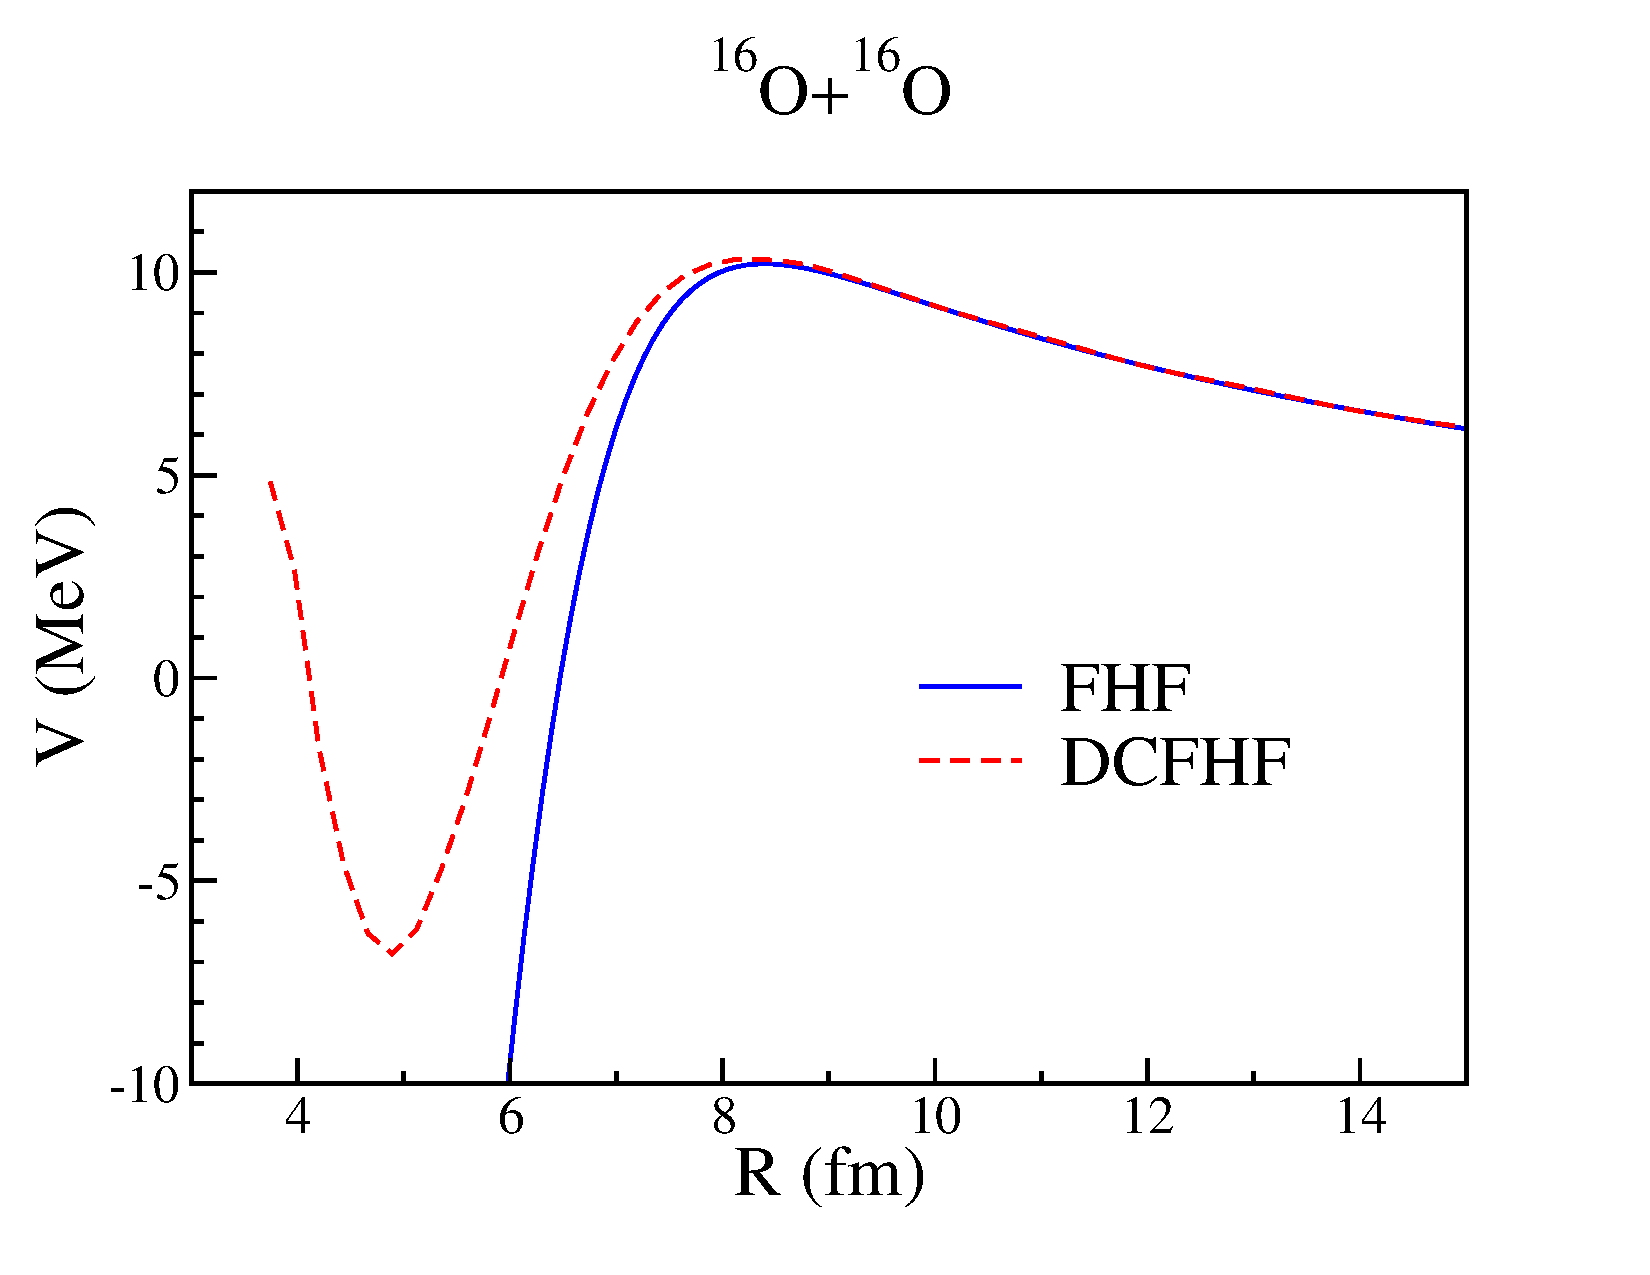
\includegraphics[width=\textwidth]{../Figures/Pauli/pot_16O+16O.pdf}
	\caption{$^{16}$O$+^{16}$O nucleus-nucleus potential without (FHF) and with (DCFHF) 
		Pauli exclusion principle between nucleons of different nuclei. }
	\label{fig:O+O}
\end{figure}

\begin{figure}
	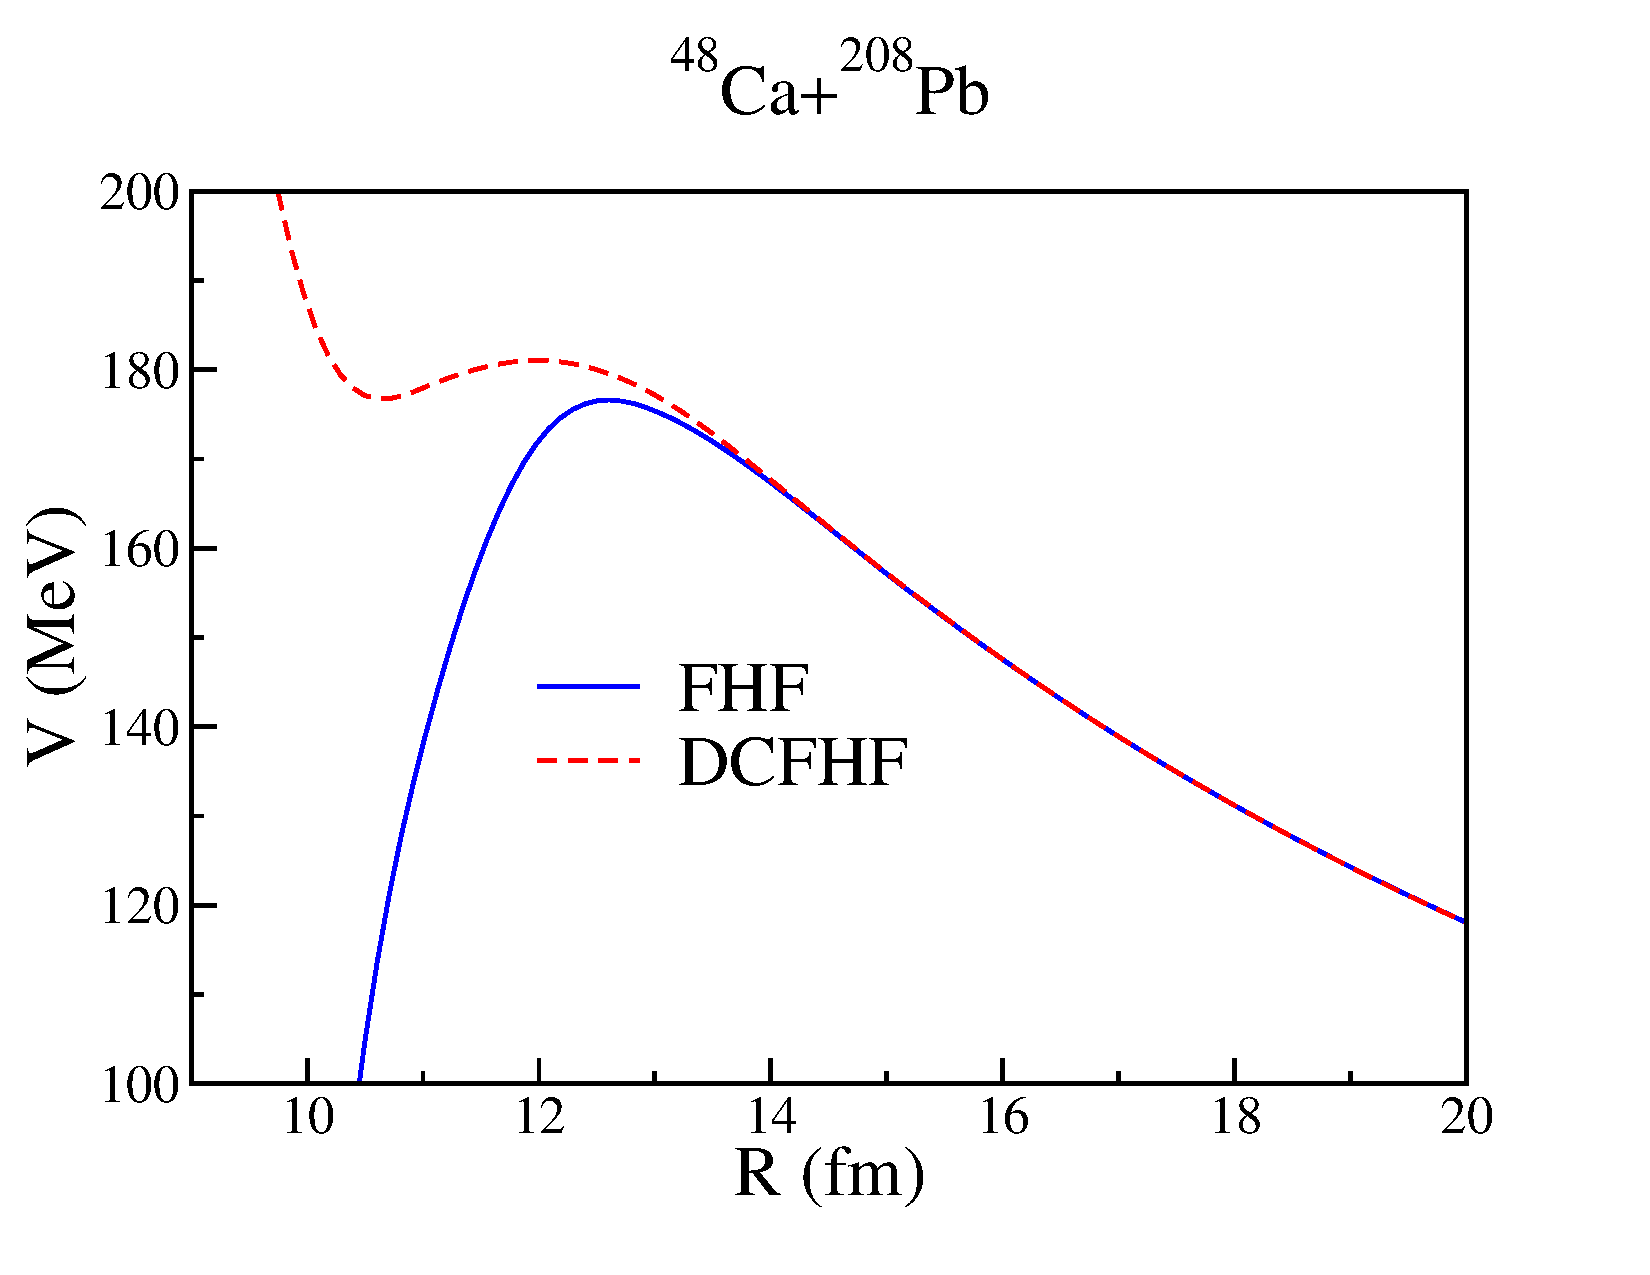
\includegraphics[width=\textwidth]{../Figures/Pauli/pot_48Ca+208Pb.pdf}
	\caption{Same as Fig.~\ref{fig:O+O} for $^{48}$Ca$+^{208}$Pb.}
	\label{fig:Ca+Pb}
\end{figure}

\section{Results}

The FHF (solid line) and DCFHF (dashed line) potentials are shown in Figs.~\ref{fig:Vb_cs}(a-c)
for $^{40}$Ca$+^{40}$Ca,   $^{48}$Ca$+^{48}$Ca, and $^{16}$O$+^{208}$Pb systems, respectively.
We observe that the Pauli exclusion principle (present only in DCFHF) induces a repulsion at short distance in the three systems.
The resulting effects are negligible outside the barrier and relatively modest near the barrier.
However, the impact is  more important in the inner barrier region, 
with the production of a potential pocket at short distance.
Interestingly, the most important effect of Pauli repulsion is to increase the barrier width. 
It is then expected to reduce the sub-barrier tunneling probability as the latter 
decreases exponentially with the barrier width.

The impact of Pauli repulsion  on the  nucleus-nucleus potential varies with the systems. 
In $^{16}$O$+^{16}$O (see Fig.~\ref{fig:O+O}), 
the pocket height is negative and Pauli repulsion is expected to have a small impact on fusion 
in this system, except potentially at astrophysical energies. 
However, the pocket becomes shallower with increasing charge product $Z_1Z_2$ 
and almost disappears in $^{48}$Ca+$^{208}$Pb (see Fig.~\ref{fig:Ca+Pb}). 
This is consistent with the fact that more nuclear overlap (and thus a larger Pauli repulsion) 
is required to compensate the larger Coulomb repulsion between the fragments. 
However, the two-body  picture for such heavy systems is questionable. 
Fig.~\ref{fig:Ca+Pb}  shows indeed an extreme case where the DCFHF calculation predicts that fusion is impossible at $3\%$ below the barrier. 
In fact, a smooth transition toward an adiabatic potential for the compound system is expected \citep{ichikawa2009b} which would allow fusion to occur at lower energies. 
Finally, the Pauli repulsion not only depends on $Z_1Z_2$, but also on the number of neutrons. 
This is illustrated in Fig.~\ref{fig:Ca+Ca} which compares the DCFHF potentials for the three $^{40,48}$Ca$+^{40,48}$Ca systems.
At touching distance, additional neutrons increase the barrier radius (due to the neutron skin) and thus decrease its height. 
For this reason, $^{48}$Ca$+^{48}$Ca has the lowest barrier and $^{40}$Ca$+^{40}$Ca the largest one. 
However, $^{48}$Ca$+^{48}$Ca also exhibits the strongest Pauli repulsion of the three systems. 
This is interpreted as an effect of the larger number of neutrons overlapping at short distance, thus increasing the Pauli repulsion. 
Note also that, once dynamics is included, fusion in these systems may behave differently and static effects on the bare potential could be washed out by the dynamics~\citep{vophuoc2016}. 
In particular, fusion in the $^{40}$Ca$+^{48}$Ca system is expected to be strongly affected by transfer channels \citep{jiang2010,montagnoli2012},  a feature which has only recently been studied in microscopic approach \citep{godbey2017}.

\begin{figure}
	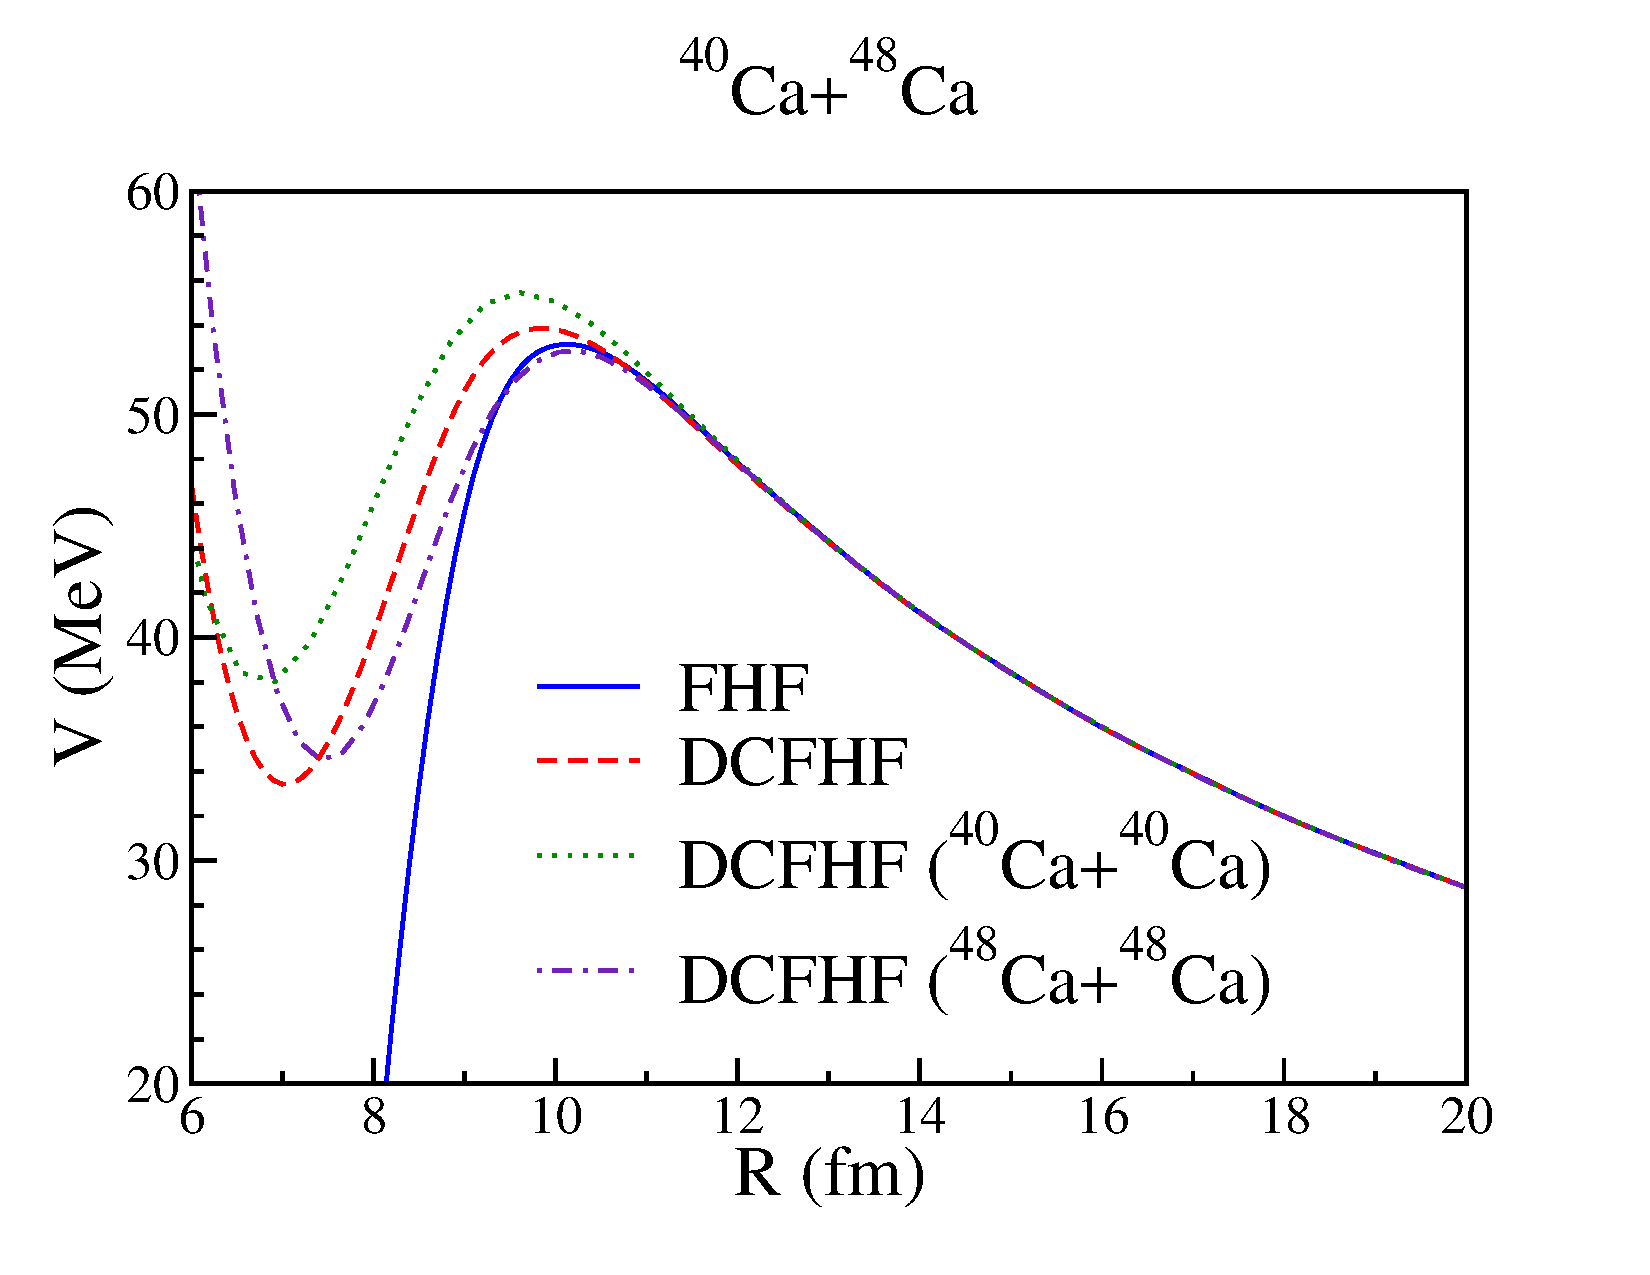
\includegraphics[width=\textwidth]{../Figures/Pauli/pot_40Ca+48Ca.pdf}
	\caption{Same as Fig.~\ref{fig:O+O} for $^{40}$Ca$+^{48}$Ca. DCFHF potentials of the other $^{A}$Ca$+^{A}$Ca are also reported.}
	\label{fig:Ca+Ca}
\end{figure}

In principle, the Pauli repulsion is expected to be energy dependent.
One source of energy dependence is the diminishing of the overlap between 
wave functions with relative kinetic momentum at higher energies
reducing the Pauli repulsion\,\citep{fliessbach1971,brink1975,goritz1976,beck1978}.
Other sources are the dependence of the EDF on the current density 
(needed for Galilean invariance)\,\citep{brink1975} and
non-local effects of the Pauli exclusion principle leading to an energy dependence 
of the local equivalent potential\,\citep{schmid1982,chamon2002}.
These effects, however, are expected to impact the Pauli repulsion at energies 
much higher than the barrier (at least twice the barrier energy in 
$^{16}$O$+^{16}$O \citep{fliessbach1971,brink1975}),
and can then be neglected in near barrier fusion studies.

We have also tested other methods to account for Pauli repulsion in the bare potential.
For instance, antisymmetrizing overlapping ground-state wave-functions
\citep{fliessbach1971,brink1975,zint1975} can be done with a Gram-Schmidt procedure.
Although the resulting potential properly accounts for the Pauli exclusion principle,
it leads to much higher repulsion as illustrated in Fig.~\ref{fig:Vb_cs}(a) (dotted-dashed line)
for the $^{40}$Ca$+^{40}$Ca system in which the potential pocket, 
and therefore the fusion barrier, simply disappear.
Let us use a simple model to explain the origin of this large repulsion.
Consider two single-particle wave functions $\az_{1,2}$ belonging to the HF ground-states of
the two different nuclei and which have a small overlap in the neck region at $\vr_0$ only:
$\az_1^*(\vr)\az_2(\vr)\simeq \alpha \delta(\vr-\vr_0)$.
By definition, the total frozen density of these two nucleons is $\rho_F=|\az_1|^2+|\az_2|^2$.
The evaluation of observables, however, requires antisymmetrized wave-functions such as
$\tilde{\az}_\pm=\mathcal{N}_{\pm}(\az_1\pm\az_2)$ with  normalization coefficients
$\mathcal{N}_\pm=(2\pm\al\pm\al^*)^{-1/2}$ and overlaps $\<\tilde\az_-|\tilde\az_+\>=0$.
The corresponding density reads
$$\tilde\rho=|\tilde\az_+|^2+|\tilde\az_-|^2\simeq\rho_F-\frac{1}{2}(\al+\al^*)^2\delta(\vr-\vr_0).$$
It is reduced in the neck compared to the frozen density and thus leads to a smaller nuclear attraction
between the nuclei or, equivalently, to a spurious repulsion between the fragments 
as seen in Fig.~\ref{fig:Vb_cs}(a).
Naive antisymmetrization procedures are then not compatible with the frozen density picture.
This was also recognized in the earlier work concerning $\alpha$-nucleus scattering studies \,\citep{fliessbach1975},
where specialized normalization operators were developed to reconstruct the states following a
Gram-Schmidt orthogonalization. However, these methods could only be applied using semi-analytic
methods. The DCFHF achieves this without any approximation.
These methods have also been subsequently criticized by groups 
performing resonating group method (RGM) calculations \citep{aoki1983,wada1987,tohsaki1975,tang1978}. 
In principle, RGM does provide a theoretical approach to construct inter nuclear 
potentials with full antisymmetrization. However, such calculations 
have thus far been limited to light systems and direct reactions due to their 
complexity. 

Let us now discuss another traditional method which is to account for Pauli repulsion
simply by increasing the kinetic energy density $\tau(\vr)$ (e.g., via the Thomas-Fermi model)
\citep{brink1975,zint1975,beck1978,denisov2010,nesterov2013}.
This method would be valid if the effect of the Pauli exclusion principle was only
to rearrange the kinetic energy term $\frac{\hb^2}{2m}\tau$ without impacting other terms of the functional.
In fact, the EDF also depends on $\tau$ via the ``$t_{1,2}$'' 
momentum dependent terms of the Skyrme  effective interaction \citep{skyrme1956}
and, then, a variation of $\tau(\vr)$ also affects the nuclear part of the potential\,\citep{brink1975,denisov2010}.
At the same time, we have also observed that including the Pauli exclusion principle 
has a strong impact on the spin-orbit energy.
This is illustrated in Fig.~\ref{fig:Vb_cs}(a) for the $^{40}$Ca$+^{40}$Ca system.
For this system, removing the spin-orbit interaction in the FHF potential  
(not shown in the figure) has little effect, but strongly increases the repulsion 
between the fragments in the DCFHF potential (thin dashed line).
This shows that the spin-orbit energy absorbs a large part of the Pauli repulsion.
Thus, the Pauli exclusion principle has a more complicated effect than just increasing the kinetic energy.

Coupled-channels calculations of fusion cross-sections 
were performed with the  \textsc{ccfull} code\,\citep{hagino1999}
using Woods-Saxon fits of the FHF and DCFHF potentials.
By default, the incoming wave boundary condition (IWBC) was used.
For shallow pocket potentials, however,
the IWBC should be replaced by an imaginary potential at the potential pocket to avoid numerical instabilities.
This is done for calculations with the $^{16}$O$+^{208}$Pb DCFHF 
potential using a modified version of \textsc{ccfull} with Woods-Saxon parameters 
$\{V_I=30$~MeV, $a_I=1$~fm, $r_I=0.3$~fm$\}$ for the imaginary potential.
Couplings to the low-lying collective $2^+$ (in calcium isotopes) and $3^-$  states are included
with standard values of the coupling constants\,\citep{morton1999,rowley2010}.
In  \textsc{ccfull}, one (two) vibrational mode(s) can be included in the projectile (target).
For the $2^+$ states, we then use the fact that, for symmetric systems,
the mutual excitation of one-phonon states in both nuclei can be approximated
by one phonon with a coupling constant scaled by $\sqrt{2}$\,\citep{esbensen1987}.
Here, the CC calculations are kept simple and include only the most relevant couplings.
Improvements could be obtained, e.g., by including anharmonicity of the multi-phonon states\,\citep{yao2016}.
The resulting fusion cross-sections are plotted in Figs.~\ref{fig:Vb_cs}(d-f). 
Calculations with the FHF potential systematically overestimate the data while the DCFHF
potential leads to a much better agreement with experiment at all energies, 
and ranging over eight orders of magnitude in cross-sections.
This shows the importance of taking into account Pauli repulsion in  the bare potential for fusion calculations.
We emphasise that these calculations are performed without adjustable parameters.

The behaviour of fusion at deep sub-barrier energies is often studied using the  logarithmic slope 
$d\ln(\sigma_{fus.}E_{c.m.})/dE_{c.m.}$. 
Large logarithmic slopes are a signature of a rapid decrease of $\sigma_{fus.}$ with decreasing energy. 
Deep-sub-barrier fusion hindrance is characterised by the failure of theoretical models 
to reproduce  large logarithmic slopes observed experimentally at low energy. 
To avoid numerical instabilities due to shallow potentials in the calculations 
of logarithmic slopes, couplings to internal excitations of the nuclei have been removed 
in the calculations of barrier transmission and accounted for via an overall lowering of $V_B$ 
by less than $5\%$ depending on the structure of the reactants \citep{dasgupta2007}. 
Indeed, it has been shown that couplings have little effects on the logarithmic slope 
at these energies \citep{dasgupta2007}. 
We see in Fig.~\ref{fig:Vb_cs}(g-i) that the inclusion of Pauli repulsion in DCFHF 
indeed increases the logarithmic slope at low energy. 

\section{Conclusion}

Although Pauli repulsion is shown to play a crucial role, it is not yet sufficient to reproduce  
experimental data at deep sub-barrier energies. 
Other contributions are expected to come from dissipative effects \citep{dasgupta2007} 
and from the transition between the nucleus-nucleus potential 
to the one-nucleus adiabatic potential\,\citep{ichikawa2009b}.
However, repulsive effects  from the incompressibility of nuclear matter 
invoked in\,\citep{misicu2006} are not observed in our microscopic calculations. 
Both the FHF and DCFHF calculations use the same Skyrme functional 
(SLy4d) with a realistic compression modulus of the symmetric nuclear 
matter $K_\infty\simeq230$~MeV. 
Although the FHF potential properly takes into account  effects due to 
incompressibility, it is very close to standard phenomenological potentials. 
We illustrate this with the example of the M3Y potential\,\citep{misicu2006} in Fig.~\ref{fig:Vb_cs}(c). 
The addition of a repulsive component at short distance [M3Y+rep parametrisation 
shown with a dotted-dashed line Fig.~\ref{fig:Vb_cs}(c)],   introduced 
phenomenologically in\,\citep{misicu2006}  to explain experimental fusion data at deep 
sub-barrier energies,  then cannot be justified by an effect of incompressibility. 
It is more likely that it simulates other effects such as  Pauli repulsion. 

C.S. thanks E. Simpson for useful discussions.
This work has been supported by the
Australian Research Council Grant No. FT120100760,
and by the U.S. Department of Energy under grant No.
DE-SC0013847 with Vanderbilt University.


\clearpage



%%
%% Chapter 4
% This is an example for a chapter, additional chapter can be added in the 
% skeleton-thesis.
% To generate the final document, run latex, build and quick build commands
% on the skeleton-thesis file not this one.

\chapter{The influence of tensor force on the microscopic heavy-ion interaction potential}\label{chapters:chapter_4}
%\vspace{-7mm}

\title{The influence of tensor force on the microscopic heavy-ion interaction potential}

\author[1,2]{Lu Guo}
\affil[1]{School of Nuclear Science and Technology, University of Chinese Academy of Sciences, Beijing 100049, China}
\affil[2]{Institute of Theoretical Physics, Chinese Academy of Sciences, Beijing 100190, China}
\author[3]{K. Godbey}
\affil[3]{Department of Physics and Astronomy, Vanderbilt University, Nashville, TN 37235}
\author[3]{A. S. Umar}


{
	\bfseries\centering

	\makeatletter

	\begin{center}
		\AB@authlist
		
		\AB@affillist
	\end{center}
	\makeatother
	
		The following work has been accepted by Physical Review C~\citep{guo2018b} and is reprinted below in its entirety.\\
	\textcopyright2018 American Physical Society\\
}
\makeatletter
\renewcommand{\AB@affillist}{}
\renewcommand{\AB@authlist}{}
\setcounter{authors}{0}
\setcounter{affil}{0}
\makeatother

\section{Abstract}

		{\bf [Background]}
		The tensor interaction is known to play an important role in the nuclear structure studies of exotic nuclei.
		However, most microscopic studies of low-energy nuclear reactions
		neglect the tensor force, resulting in a lack of knowledge concerning the effect of the tensor force on heavy-ion collisions.
		An accurate description of the heavy-ion interaction
		potential is crucial for understanding the microscopic mechanisms of heavy-ion fusion dynamics.
		Furthermore, the building blocks of the heavy-ion interaction potential in terms of the ingredients of the
		effective nucleon-nucleon interaction provides the physical underpinnings for connecting the theoretical
		results with experiment.
		The tensor force has never been
		incorporated for calculating the nucleus-nucleus interaction potential.
		
		{\bf [Purpose]}
		The theoretical study of the influence of the tensor force on heavy-ion interaction potentials is required to further our
		understanding of the microscopic mechanisms entailed in fusion dynamics.
		
		{\bf [Method]}
The full Skyrme tensor force is implemented into the static Hartree-Fock and dynamic density-constrained time-dependent Hartree-Fock
(DC-TDHF) theory
to calculate both static (frozen density) and dynamic microscopic interaction potentials for reactions involving exotic and stable nuclei.
		
		{\bf [Results]}
The static potentials are found to be systematically higher than the dynamical results, which are attributed to the microscopic dynamical effects included in TDHF.
We also show that the dynamical potential barriers vary more significantly by the inclusion of tensor force than the static barriers.
The influence of isoscalar and isovector tensor terms is also investigated with the T$IJ$ set of forces.
For light systems, the tensor force is found to have an imperceptible effect on the nucleus-nucleus potential. However, for medium and heavy spin-unsaturated reactions,
the potentials may change from a fraction of an MeV to almost 2~MeV by the inclusion of tensor force, indicating a strong impact of the tensor force on sub-barrier fusion.
		
		{\bf [Conclusions]}
		The tensor force could indeed play a large role in the fusion of nuclei, with spin-unsaturated systems seeing a systematic increase in ion-ion barrier height and width. This fusion hindrance is partly due to static, ground state effects from the inclusion of the tensor force, though additional hindrance appears when studying nuclear dynamics.




% insert suggested PACS numbers in braces on next line
%\pacs{}
% insert suggested keywords - APS authors don't need to do this
%\keywords{}

%\maketitle must follow title, authors, abstract, \pacs, and \keywords

%\end{CJK*}

\section{Introduction}
\label{introduction}

With the increasing availability of radioactive ion beams, the study of structure and reactions of exotic nuclei is
one of the most fascinating research areas in nuclear physics~\citep{Balantekin2014_MPLA29-1430010}.
The exotic nuclei display distinct features from those seen in typical stable nuclei, which is attributed partly to the unique characteristics of the nucleon-nucleon interaction.
The tensor interaction between nucleons is one such characteristic and is well known to be important in nuclear structure
properties~\citep{Lesinski2007_PRC76-014312}, e.g.,
the shell evolution of exotic nuclei~\citep{Otsuka2006_PRL97-162501},
spin-orbit splitting~\citep{Colo2007_PLB646-227}, and Gamow-Teller and charge exchange spin-dipole excitations~\citep{Bai2010_PRL105-072501}.
However, its role in low-energy nuclear reactions is poorly understood as the tensor force has been neglected in most reaction dynamics calculations.
In particular, regarding nuclear dynamics, the tensor force changes not only the spin-orbit splitting but also the intrinsic excitations which may give rise to dynamical effects which are more complicated than those arising from simple shell evolution.
The study of the effects of the tensor force on heavy-ion fusion dynamics will lead to a better understanding of the effective nucleon-nucleon interaction and of the correlations present in these many-body systems.

The study of heavy-ion interaction potentials is of fundamental importance for above barrier and sub-barrier fusion reactions~\citep{Back2014_RMP86-317}.
In general, two categories of theoretical approaches are used for
calculating ion-ion potentials. In the first category, phenomenological models such as the Bass model~\citep{Bass1974_NPA231-45}, the proximity potential~\citep{Randrup1978_PLB77-170,Seiwert1984_PRC29-477}, the double-folding potential~\citep{Satchler1979_PR55-183,Rhoades-Brown1983_PRL50-1435}, and driven potential from dinuclear system model~\citep{Adamian2004_PRC69-044601,
	Wang2012_PRC85-041601,Zhu2016_PRC93-064610,Bao2016_PRC93-044615,Feng2018_PRC95-024615} could be mentioned.
Although these methods have been successful in explaining particular aspects of reaction
data~\citep{Randrup1978_NPA307-319,Fazio2004_EPJA19-89}, the uncertainty of macroscopic parameters and the lack of microscopic origins restrict their predictive power and may obscure the underlying physical processes.
Second category contains the semi- and fully microscopic approaches to obtain potentials by including the interactions of the constituents~\citep{Moller2004_PRL92-072501,Guo2004_NPA740-59,Guo2005_PRC71-024315,Guo2007_PRC76-034317,Lu2014_PRC89-014323}.
One common  assumption used in many of the semi-microscopic calculations is that of the frozen density or sudden approximation~\citep{Brueckner1968_PR173-944}, in which the nuclear densities are unchanged during the computation of the nucleus-nucleus potential as a function of internuclear distance.
This approximation may result in an unphysical potential at deep sub-barrier energies, where the inner turning point of the interaction potential corresponds to large nuclear overlap.
Various remedies have been developed to address this issue within the confines of the coupled-channels approach~\citep{Misicu2006_PRL96-112701,Ichikawa2007_PRC75-057603}.
In other microscopic approaches, such as the constrained mean-field methods, although the nuclear densities are allowed for the rearrangement, the potential energy path is obtained by the static adiabatic approximation, thus ignoring the dynamical effects.

In recent years we have developed the density-constrained time-dependent Hartree-Fock (DC-TDHF) approach for calculating heavy-ion interaction
potentials, which naturally incorporate all of the dynamical effects included in the time-dependent Hartree-Fock (TDHF) description of the collision process~\citep{Umar2006_PRC74-021601}.
These effects include nucleon transfer, couplings between the collective motion and intrinsic degrees of freedom, neck formation, internal excitations, and deformation effects to all orders.
The method is based on the TDHF evolution of the nuclear dynamics coupled with density-constrained (DC) Hartree-Fock (HF) calculations to obtain the ion-ion potential.
In contrast to other mean-field based microscopic methods, the DC-TDHF approach doesn't need
to introduce external constraining operators which assume that the collective motion is confined to the constrained phase space. That means that the many-body system
selects its evolutionary path by itself following the microscopic dynamics. We have applied this method for a wide range of reactions ~\citep{Umar2006_PRC74-024606,Umar2006_PRC74-061601,Umar2008_PRC77-064605,Umar2008_EPJA37-245, Umar2009_PRC80-041601,Oberacker2010_PRC82-034603,Keser2012_PRC85-044606,Umar2012_PRC85-055801,
	Umar2014_PRC89-034611,Godbey2017_PRC95-011601} and found reasonable agreement between the measured fusion cross sections and the DC-TDHF results.
To our knowledge, neither the phenomenological nor microscopic methods for calculating ion-ion potential include the tensor
force between nucleons, which is an important component of the nuclear force. Our work is the first attempt to investigate the effect induced by the tensor
force on heavy-ion interaction potentials.

The TDHF approach is a well-defined framework and provides a useful foundation for a fully microscopic many-body theory.
Quantum effects are considered, which is essential for the manifestation of shell effects during the collision dynamics.
Recently, the effect of the tensor force in heavy-ion collisions has been studied using direct TDHF calculations~\citep{Fracasso2012_PRC86-044303,Dai2014_SciChinaPMA57-1618,Stevenson2016_PRC93-054617,Shi2017_NPR34-41,Guo2018_PLB782-401}.
Furthermore, the TDHF approach provides a deeper understanding of nuclear dynamics, as seen in recent applications to fusion~\citep{Simenel2004_PRL93-102701,Umar2009_PRC80-041601,Oberacker2010_PRC82-034603,Guo2012_EPJWoC38-09003,
	Keser2012_PRC85-044606,Umar2012_PRC85-055801,Simenel2013_PRC88-024617,
	Umar2014_PRC89-034611,Washiyama2015_PRC91-064607,Tohyama2016_PRC93-034607,Godbey2017_PRC95-011601,Simenel2017_PRC95-031601},
quasifission~\citep{Golabek2009_PRL103-042701,Oberacker2014_PRC90-054605,Umar2015_PRC92-024621,Umar2016_PRC94-024605,Yu2017_SciChinaPMA60-092011}, transfer reactions~\citep{Washiyama2009_PRC80-031602,Simenel2010_PRL105-192701,Simenel2011_PRL106-112502,Scamps2013_PRC87-014605,Sekizawa2013_PRC88-014614,
	Wang2016_PLB760-236,Sekizawa2016_PRC93-054616,Sekizawa2017_PRC96-041601},
fission~\citep{Simenel2014_PRC89-031601,Scamps2015_PRC92-011602,Goddard2015_PRC92-054610,Goddard2016_PRC93-014620,Bulgac2016_PRL116-122504,Tanimura2017_PRL118-152501},
and deep inelastic collisions~\citep{Maruhn2006_PRC74-027601,Guo2007_PRC76-014601,Guo2008_PRC77-041301,Iwata2011_PRC84-014616,Dai2014_PRC90-044609,Dai2014_SciChinaPMA57-1618,
	Stevenson2016_PRC93-054617,Guo2017_EPJWoC163-00021,Shi2017_NPR34-41,Umar2017_PRC96-024625}.
%and resonance dynamics~\citep{Simenel2001_PRL86-2971,
%Simenel2003_PRC68-024302,Maruhn2005_PRC71-064328,Nakatsukasa2005_PRC71-024301,Umar2005_PRC71-034314,Reinhard2007_EPJA32-19,Simenel2009_PRC80-064309,
%Fracasso2012_PRC86-044303,Avez2013_EPJA49-76,Ebata2014_PRC90-024303}.
For recent reviews see Refs.~\citep{Simenel2012_EPJA48-152,Nakatsukasa2016_RMP88-045004,Simenel2018_PPNP}.

This article is organized as follows. In Sec.~\ref{tenpot:theory}, we summarize the theoretical formalism of Skyrme energy functional with the tensor force included and the TDHF and DC-TDHF approaches.
Section~\ref{discuss} presents the systematic analysis of the impact of the tensor force on heavy-ion interaction potentials.
A summary is given in Sec.~\ref{summary}.

\section{Theoretical framework}
\label{tenpot:theory}

Despite the wide application of the TDHF approach, various assumptions and approximations that may affect the TDHF results have been employed in the past.
This led to an occasional imperfect or even incorrect reproduction of experimental data.
To remedy these problems a considerable theoretical and computational effort has been undertaken for increased numerical accuracy
and improved effective interactions.
For instance, the inclusion of the spin-orbit interaction solved an early conflict between TDHF predictions and experimental observations~\citep{Umar1986_PRL56-2793,Umar1989_PRC40-706} and turned out to play an important role in fusion and dissipation dynamics~\citep{Maruhn2006_PRC74-027601,Dai2014_PRC90-044609}. In recent years it has become feasible
to perform TDHF calculations on a three-dimensional Cartesian grid without any symmetry restrictions and with accurate numerical methods. In
addition, the quality of energy density functional (EDF) has been substantially improved. The time-odd
terms in particular have shown to be non-negligible in heavy-ion collisions~\citep{Umar2006_PRC73-054607}. However, there are still important components of the basic theory that have not yet been fully implemented, such as the tensor force between nucleons. In order to study the role of tensor force
in heavy-ion interaction potential, we incorporate the full tensor force into the microscopic TDHF
and DC-TDHF approaches.

\subsection{Full Skyrme energy functional}

Most TDHF calculations employ the Skyrme effective interaction~\citep{Skyrme1956_PM1-1043}, in which the two-body tensor force was proposed in its original form as
\begin{align}
\begin{split}
v_T&=\dfrac{t_\mathrm{e}}{2}\bigg\{\big[3({\sigma}_\mathrm{1}\cdot\mathbf{k}')({\sigma}_\mathrm{2}\cdot\mathbf{k}')-({\sigma}_\mathrm{1}\cdot{\sigma}_\mathrm{2})\mathbf{k}'^{\mathrm{2}}\big]\delta(\mathbf{r}_\mathrm{1}-\mathbf{r}_\mathrm{2})\\
&+\delta(\mathbf{r}_\mathrm{1}-\mathbf{r}_\mathrm{2})\big[3({\sigma}_\mathrm{1}\cdot\mathbf{k})({\sigma}_\mathrm{2}\cdot\mathbf{k})-({\sigma}_\mathrm{1}\cdot{\sigma}_\mathrm{2})\mathbf{k}^\mathrm{2}\big]\bigg\}\\
&+t_\mathrm{o}\bigg\{3({\sigma}_\mathrm{1}\cdot\mathbf{k}')\delta(\mathbf{r}_\mathrm{1}-\mathbf{r}_\mathrm{2})({\sigma}_\mathrm{2}\cdot\mathbf{k})-({\sigma}_\mathrm{1}\cdot{\sigma}_\mathrm{2})\mathbf{k}'
\delta(\mathbf{r}_\mathrm{1}-\mathbf{r}_\mathrm{2})\mathbf{k}\bigg\}.
\end{split}
\end{align}
The coupling constants $t_\textrm{e}$ and $t_\textrm{o}$ represent the strengths of triplet-even and
triplet-odd tensor interactions, respectively.  The operator $\mathbf{k}=\frac{1}{2i}(\nabla_1-\nabla_2)$ acts on the right and
$\mathbf{k}'=-\frac{1}{2i}(\nabla'_1-\nabla'_2)$ acts on the left.

It is natural to represent the total energy of the system
\begin{equation}
E=\int d^3r  {\cal H}(\rho, \tau, {\mathbf{j}}, {\textbf{s}}, {\textbf{T}}, {\textbf{F}}, J_{\mu\nu}; {\mathbf{r}})
\label{Energy}
\end{equation}
in terms of the energy functional. The functional is composed by
the number density $\rho$, kinetic density $\tau$, current density ${\mathbf{j}}$, spin density ${\mathbf{s}}$, spin-kinetic density ${\mathbf{T}}$,
the tensor-kinetic density {\textbf{F}}, and spin-current pseudotensor density $J$~\citep{Stevenson2016_PRC93-054617}. The full version of Skyrme EDF is expressed as
\begin{align}
\label{EDFH}
\begin{split}
\mathcal{H}&=\mathcal{H}_0+\sum_{\rm{t=0,1}}\Big\{A_{\rm{t}}^{\rm{s}}\mathbf{s}_{\rm{t}}^2+(A_{\rm{t}}^{\Delta{s}}+B_{\rm{t}}^{\Delta{s}})
\mathbf{s}_{\rm{t}}\cdot\Delta\mathbf{s}_{\rm{t}}+B_{\rm{t}}^{\nabla s}(\nabla\cdot \mathbf{s}_{\rm{t}})^2 \\
&+B_{\rm{t}}^{F}\big(\mathbf{s}_{\rm{t}}\cdot
\mathbf {F}_{\rm{t}}-\frac{1}{2}\big(\sum_{\mu=x}^{z}J_{\rm{t}, \mu\mu}\big)^2-\frac{1}{2}\sum_{\mu, \nu=x}^{z}J_{\rm{t}, \mu\nu}J_{\rm{t}, \nu \mu}\big)\\
&+(A_{\rm{t}}^{\rm{T}}+B_{\rm{t}}^{\rm{T}})\big(\mathbf{s}_{\rm{t}}\cdot\mathbf{T}_{\rm{t}}-
\sum_{\mu,\nu=x}^{z}J_{\rm{t},\mu\nu}J_{\rm{t},\mu\nu}\big)\Big\},
\end{split}
\end{align}
where $\mathcal{H}_0$ is the simplified functional used in the Sky3D TDHF code~\citep{Maruhn2014_CPC185-2195} and most TDHF calculations.
The terms containing the coupling constants $A$ arise from the Skyrme central force and those with $B$ from the tensor force. The definitions of both $A$ and $B$
can be found in Refs.~\citep{Lesinski2007_PRC76-014312,Davesne2009_PRC80-024314}. All the time-even and time-odd terms in Eq.~(\ref{EDFH}) have been implemented numerically in the mean-field Hamiltonians of the HF, TDHF and
DC-TDHF approaches.
As pointed out in Refs.~\citep{Lesinski2007_PRC76-014312,Stevenson2016_PRC93-054617}, the terms containing the gradient of spin density may cause spin instability in both nuclear structure and reaction studies, hence the terms of $\mathbf{s}_{\rm{t}}\cdot\Delta\mathbf{s}_{\rm{t}}$ and $(\nabla\cdot \mathbf{s}_{\rm{t}})^2$ have been turned off in all calculations.

\subsection{TDHF approach}

Given a many-body Hamiltonian, the action can be constructed as
\begin{equation}
S=\int_{t_1}^{t_2} dt \langle \Phi(\textbf{r}, t)|H-i\hbar \partial_t|\Phi(\textbf{r}, t)\rangle ,
\end{equation}
where $\Phi$ is the time-dependent many-body wave function.
In TDHF approach the many-body wave function $\Phi(\mathbf{r}, t)$ is approximated as a single time-dependent Slater determinant composed of an antisymmetrized product
of the single particle states $\phi_{\rm{\lambda}}(\mathbf{r}, t)$
\begin{equation}
\Phi(\mathbf{r}, t)=\frac{1}{\sqrt{N!}}\textrm{det}\{\phi_{\rm{\lambda}}(\mathbf{r}, t)\},
\end{equation}
and this form is kept at all times in the dynamical evolution.
By taking the variation of the action with respect to the single-particle wave functions, the set of nonlinear coupled TDHF equations in the multidimensional
space-time phase space
\begin{equation}
i\hbar \frac{\partial}{\partial_t}\phi_{\rm{\lambda}}(\mathbf{r}, t)=h\phi_{\rm{\lambda}}(\mathbf{r}, t)
\end{equation}
yields the most probable time-dependent mean-field path, where $h$ is the HF single-particle Hamiltonian.
The set of nonlinear TDHF equations has been solved on three-dimensional
coordinate space without any symmetry restrictions and with modern, accurate numerical methods~\citep{Umar2006_PRC73-054607,Maruhn2014_CPC185-2195}.

\subsection{Dynamical potential from DC-TDHF approach}

Since TDHF theory describes the collective motion of fusion dynamics in terms of semi-classical trajectories, the sub-barrier quantum
tunneling of the many-body wave function can not be included. Consequently, direct TDHF calculations can not be used to describe sub-barrier fusion.
At present, all sub-barrier fusion calculations assume that there exists an ion-ion potential which depends on the internuclear distance.
The microscopic DC-TDHF approach~\citep{Umar2006_PRC74-021601} is employed to extract the nucleus-nucleus potential from the TDHF time evolution of the dinuclear system.
In this approach, at certain time during the evolution, the instantaneous TDHF density is used to perform a static HF energy minimization
\begin{equation}
\delta \langle \Psi_{\rm DC}|H-\int d^3r \lambda(\textbf{r})\rho(\textbf{r})|\Psi_{\rm DC}\rangle=0,
\end{equation}
by constraining the proton and neutron densities to be equal to the instantaneous TDHF densities. Since we are constraining the total density,
all moments are simultaneously constrained. DC-TDHF calculations give the adiabatic reference state for a given TDHF state, which is the Slater
determinant with the lowest energy for a given density.
The minimized energy
\begin{equation}
E_{\rm {DC}}(\textbf R)=\langle \Psi_{\rm DC}|H|\Psi_{\rm DC}\rangle
\end{equation}
is the density-constrained energy.
Since this density-constrained potential still contains the binding energies of individual nuclei which should be subtracted out,
the heavy-ion interaction potential is deduced as
\begin{equation}
V(\textbf R)=E_{\rm {DC}}(\textbf R)-E_{\rm {A1}}-E_{\rm {A2}},
\label{VB}
\end{equation}
where $E_{\rm {A1}}$ and $E_{\rm {A2}}$ are the binding energies of the two individual nuclei.
One should note that this procedure does not affect the TDHF time evolution and contains no free parameters or normalization.

\subsection{Bare potential from FHF approach}

In previous subsection, the DC-TDHF technique has been introduced to compute the nucleus-nucleus potential in a dynamical microscopic way.
All of the dynamical effects included in TDHF is then directly incorporated in the potential. Here we look for a different approach
to produce a bare potential which does not include any dynamical contribution, since we aim to disentangle the static and dynamical effects
of the tensor force. The bare nucleus-nucleus potential is defined as the interaction potential between the nuclei in their ground states.
In addition, to preserve the consistency with microscopic calculations, it is necessary to compute the potential from the same EDF used in
HF, TDHF, and DC-TDHF calculations. This is possible using the frozen Hartree-Fock (FHF) technique~\citep{Simenel2013_PRC88-064604},
assuming that the densities of the target and
projectile remain constant and equal to their respective ground state densities.
The potential can then be expressed as
\begin{align}
\label{eq:FD}
V_\mathrm{FD}(\textbf R)=E[\rho_\mathrm{1}+\rho_\mathrm{2}](\textbf R)-E[\rho_\mathrm{1}]-E[\rho_\mathrm{2}],
\end{align}
where $\rho_\mathrm{1}$ and $\rho_\mathrm{2}$ are HF ground state densities of the fragments, and $E[\rho_\mathrm{1}+\rho_\mathrm{2}]$ is the same
Skyrme EDF as defined in Eqs.~(\ref{Energy}) and (\ref{EDFH}). In the FHF approach, the Pauli principle between pairs of nucleons belonging to different
collision partners has been neglected. When the overlap between the density distributions is small, the barrier is almost unaffected by the inclusion of the Pauli principle.
However, at larger overlaps of the densities where the Pauli principle is expected to play a more important role, the FHF approximation may not properly
account for the potential, particularly the inner part~\citep{Simenel2017_PRC95-031601}.

\section{Results}
\label{discuss}

The concept of using density as a constraint for calculating collective states from TDHF time evolution was first introduced in the mid 1980s~\citep{Cusson1985_ZPA320-475}, and was used for the microscopic description of nuclear molecular resonances~\citep{Umar1985_PRC32-172}.
In recent years, the DC-TDHF approach has demonstrated its feasibility and success in explaining sub-barrier fusion dynamics for a wide range of reactions.
This is rather remarkable given the fact that the only input in DC-TDHF is the Skyrme effective interaction, and there are no adjustable parameters.
In the present work, we focus on how the tensor force affect the nucleus-nucleus potential which is vital for the theoretical analysis of sub-barrier fusion dynamics.
We have thus chosen ten representative reactions with proton and neutron numbers of reaction partners corresponding to the magic numbers 8, 20, 28, 50, and 82,
in which the spin-saturated shells are 8 and 20.

In the numerical simulation the static HF ground state for the reaction partner has been calculated on the symmetry-unrestricted three-dimensional grid.
The resulting Slater determinants for each nucleus comprise the larger Slater determinant describing the colliding system during the dynamical evolution.
The TDHF time propagation is performed using a Taylor-series expansion up to the sixth order of the unitary boost operator with
a time step of $0.2 ~\mathrm {fm}/c$. For the dynamical evolution, we use a numerical box of 48 fm along the collision axis and 24 fm in the
other two directions and a grid spacing of 1.0~fm. The initial separation between the two nuclei is 20~fm. The choice of these
parameters assures good numerical accuracy in the unrestricted TDHF evolution. We have simultaneously performed the density constraint
calculations utilizing the DC-TDHF method at every 10-20 time steps (corresponding to 2-4~$\mathrm {fm}/c$ interval).
The convergence property in DC-TDHF calculations is as good if
not better than in the traditional constrained HF with a constraint on a single collective degree of freedom.

We employ the Skyrme interaction in the calculations, in which the tensor force has been constructed in two ways.
One is to add the force perturbatively to the existing standard interactions, for instance,
the existing Skyrme parameter SLy5~\citep{chabanat1998a} plus tensor force, denoted as SLy5t~\citep{colo2007}.
The comparison between calculations with SLy5 and SLy5t addresses the question on how much of the changes is caused by tensor force itself.
Another approach is to readjust the full set of Skyrme parameters self-consistently.
This strategy has been adopted in Ref.~\citep{Lesinski2007_PRC76-014312} and led to
the set of T$IJ$ parametrizations with a wide range of isoscalar and isovector tensor couplings.
Due to its fitting strategy, the contributions from the tensor force and the rearrangement of all other terms could be physically entangled.
\begin{figure}
	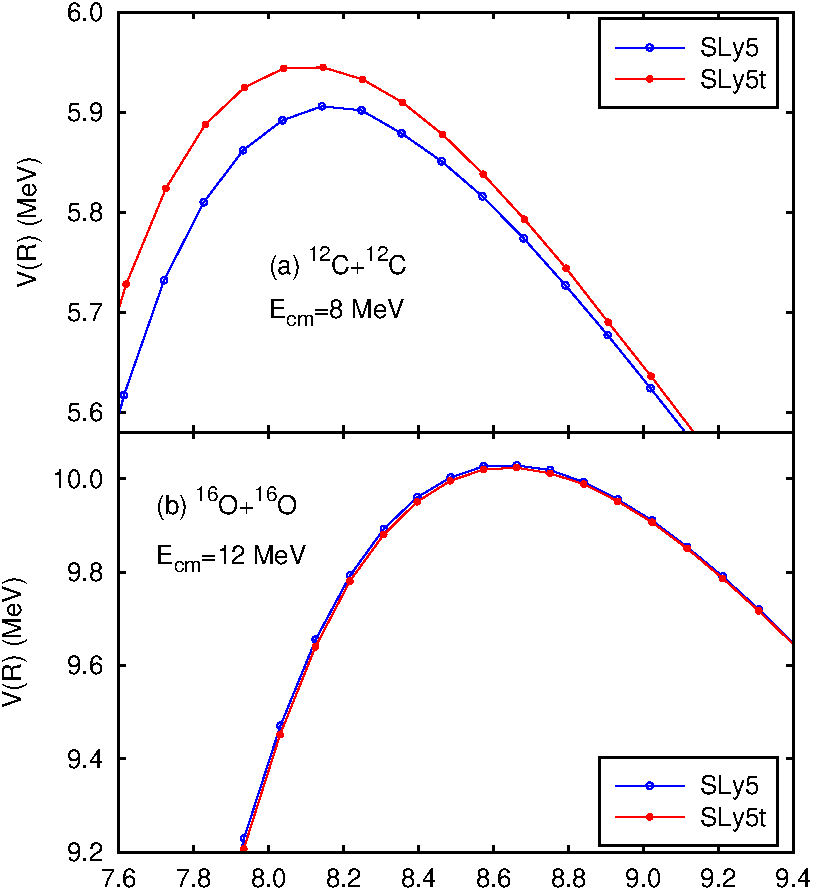
\includegraphics[width=\textwidth]{../Figures/TensorPot/V1.pdf}
	\caption{Internuclear potential obtained from DC-TDHF approach shown for the evolution of the systems (a) $^{12}\mathrm{C}+\mathrm{^{12}C}$
		at $E_{\mathrm{c.m.}}=8$ MeV  and (b) $^{16}\mathrm{O}+\mathrm{^{16}O}$ at $E_{\mathrm{c.m.}}=12$ MeV with SLy5 (open circle) and SLy5t (solid circle) forces.
		\label{Fig:light}}
\end{figure}

\begin{figure}
	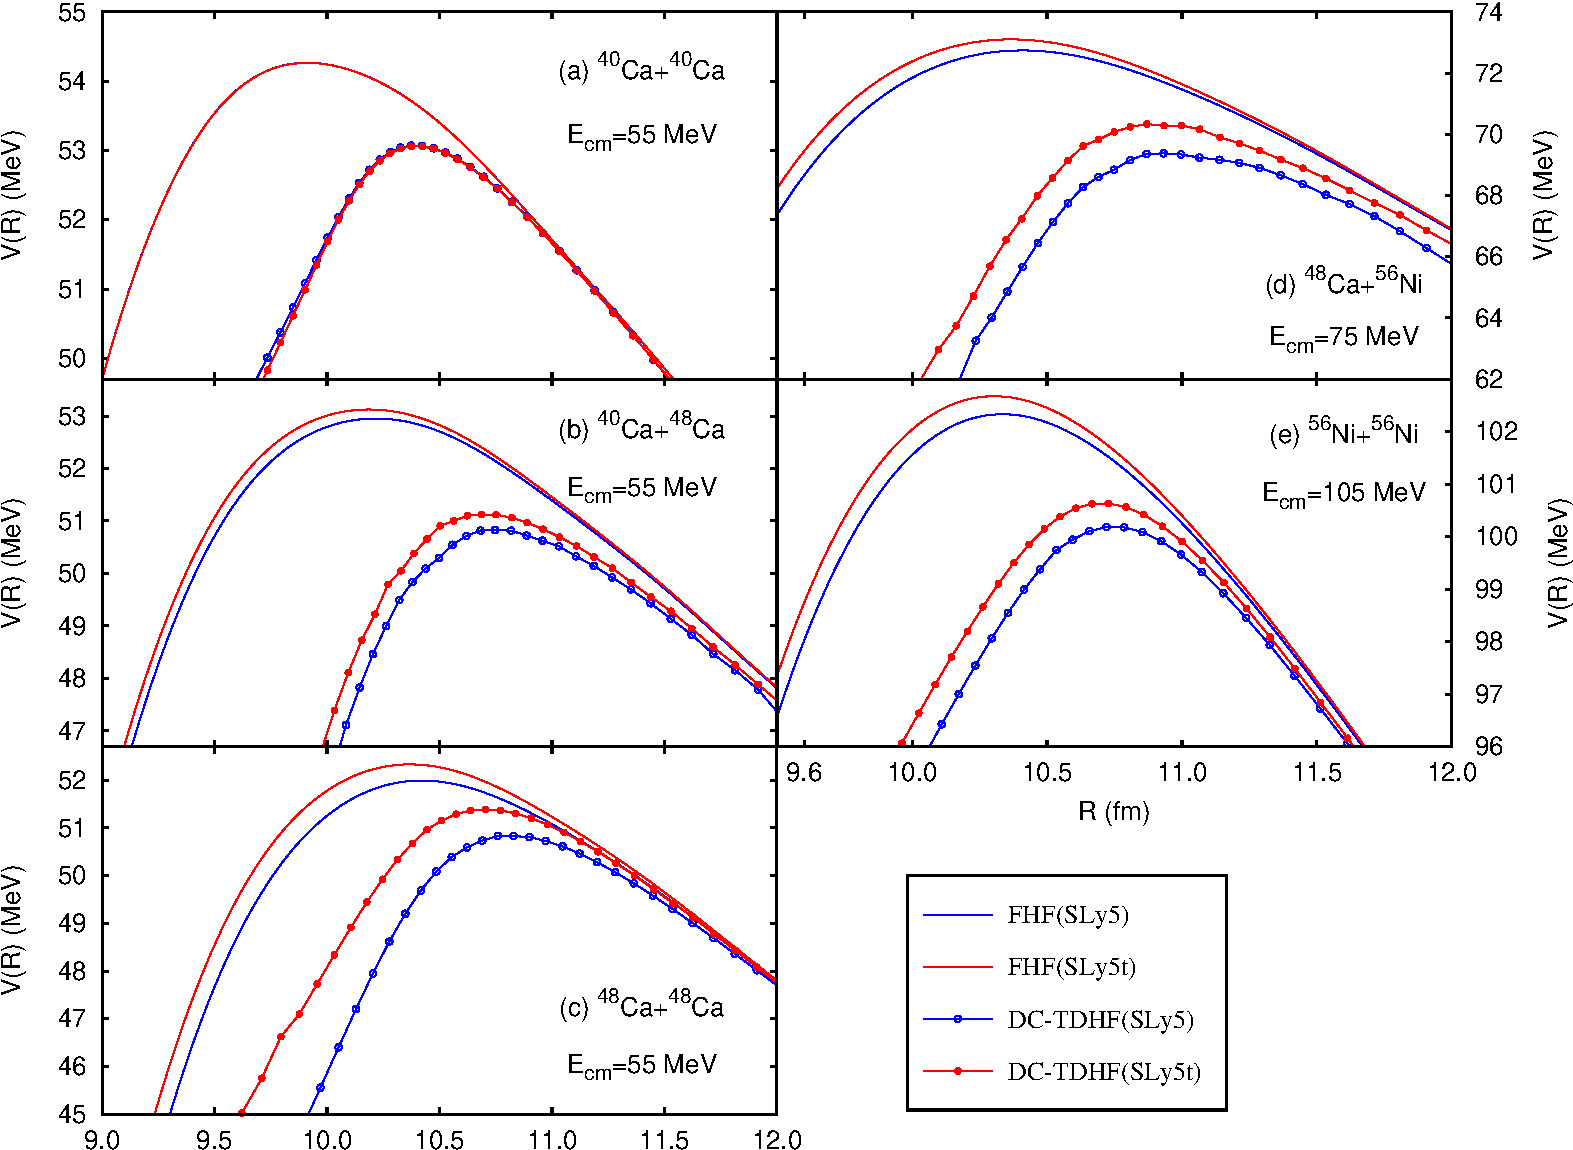
\includegraphics[width=\textwidth]{../Figures/TensorPot/V3_ppt.pdf}
	\caption{Internuclear potential obtained from FHF and DC-TDHF approaches for the Ca+Ca, Ca+Ni, and Ni+Ni reactions
		with tensor (SLy5t) and without tensor (SLy5) forces.
		\label{Fig:medium}}
\end{figure}

For light systems, we choose the spin-unsaturated $^{12}\mathrm{C}+\mathrm{^{12}C}$ and spin-saturated $^{16}\mathrm{O}+\mathrm{^{16}O}$ reactions
for comparison. As we have reported in Ref.~\citep{Umar2014_PRC89-034611}, the potential barriers are sensitive to the
colliding energy. Hence, the same initial energy, close to the Coulomb barrier, is used for the reaction with and without tensor forces.
In Fig.~\ref{Fig:light}, we plot the ion-ion potentials obtained from Eq.~(\ref{VB}) using the DC-TDHF approach for (a) $^{12}\mathrm{C}+\mathrm{^{12}C}$
at $E_{\mathrm{c.m.}}=8$ MeV  and (b) $^{16}\mathrm{O}+\mathrm{^{16}O}$ at $E_{\mathrm{c.m.}}=12$ MeV with SLy5 (open circle) and SLy5t (solid circle) forces.
Both nuclei, $^{12}\mathrm{C}$ and $\mathrm{^{16}O}$, show spherical ground states with tensor (SLy5t) and without tensor (SLy5) forces, which
are in agreement with experimental data and other calculations. The correct description of the initial shape of
target and projectile nucleus is important for the dynamical evolution of heavy-ion collisions.
We see that for the spin-unsaturated system $^{12}\mathrm{C}+\mathrm{^{12}C}$, the potential with the tensor force included has an overall higher
interaction barrier than without the tensor force, although the difference of the potential barrier peak is small at roughly 0.07~MeV.
For the spin-saturated system $^{16}\mathrm{O}+\mathrm{^{16}O}$, the internuclear potential is close with and without tensor force,
having a barrier height of 10.02~MeV and a peak location of 8.66~fm. This indicates that the tensor force has negligible effect on the near-barrier fusion
for the spin-saturated system $^{16}\mathrm{O}+\mathrm{^{16}O}$, which is consistent with the findings in Ref.~\citep{Stevenson2016_PRC93-054617}.
For these light systems the tensor force shows a small effect on the interaction potential.



For reactions involving two medium mass nuclei, we have chosen five representative reactions $^{40}\mathrm{Ca}+\mathrm{^{40}Ca}$,
$^{40}\mathrm{Ca}+\mathrm{^{48}Ca}$, $^{48}\mathrm{Ca}+\mathrm{^{48}Ca}$, $^{48}\mathrm{Ca}+\mathrm{^{56}Ni}$, and $^{56}\mathrm{Ni}+\mathrm{^{56}Ni}$,
which vary by the total number of spin-unsaturated magic numbers in target and projectile by 0, 1, 2, 3, and 4.
In these collisions, the reaction partners are closed-shell corresponding to 20 (spin-saturated) and 28 (spin-unsaturated) neutron or proton magic numbers.
To disentangle the static (e.g. modification of ground-state density) and dynamical (e.g. modification of couplings, dissipation, and transfer) origins of the tensor
force, the nucleus-nucleus potentials obtained both from FHF and DC-TDHF calculations are shown in Fig.~\ref{Fig:medium} for all Ca and Ni reactions.
In the initial state of the collision dynamics, the deviation of the static FHF potential from the dynamical DC-TDHF result is the order of smaller than 10 keV.
For all the Ca and Ni reactions, we observe that the nucleus-nucleus potentials are considerably different for the static FHF and dynamical DC-TDHF results.
The static potentials are systematically higher than the dynamical results, and the barrier peaks are located at smaller relative distance with FHF. In particular,
the inner part of the potential, having strong effect on the sub-barrier fusion, presents more significant difference for FHF and DC-TDHF results.
This behavior is well understood and is a consequence of the absence of Pauli principle and excitations for the frozen density overlaps in FHF
potentials~\citep{Simenel2013_PRC88-064604,Guo2018_PLB782-401,Simenel2017_PRC95-031601}, thus the difference between FHF and DC-TDHF is due to dynamical effects.
Another interesting observation is that the variation of dynamical barriers due to tensor force is systematically greater than the
ones for the static barriers.
This indicates that the tensor force influences not only
the ground-state single-particle levels, but also the dynamical effects including nucleon transfer, the couplings to low-lying states, and intrinsic
excitations.
In Ref.~\citep{Guo2018_PLB782-401}, how these dynamical effects affect the fusion barriers heights, computed directly from TDHF, have been investigated to study the
role of tensor force on above-barrier fusion dynamics.
We note that in Ref.~\citep{Guo2018_PLB782-401}, for the $^{48}\mathrm{Ca}+\mathrm{^{56}Ni}$ system, the
tensor force was observed to decrease the barrier height in direct TDHF calculations, which is the opposite of
the trend observed here.
This difference might arise from the dynamical energy-dependent effects introduced by the tensor force that
are not captured by the DC-TDHF potential.



For the spin-saturated reaction $^{40}\mathrm{Ca}+\mathrm{^{40}Ca}$, the interaction potential remains nearly unchanged by the inclusion of tensor force
for both static and dynamical cases, indicating that the tensor force has almost no impact on the dynamical evolution for spin-saturated systems,
since the contribution of tensor force is expected to be nearly zero for the ground state of spin-saturated nuclei.
For the spin-unsaturated reactions, the barriers with tensor force SLy5t are systematically higher than those without the tensor force SLy5.
This indicates a fusion hindrance effect due to the tensor force in this mass region. Empirically, 1 MeV larger in the inner part of the potential barrier
can cause one order lower in the fusion cross section at sub-barrier energies. From the comparison of dynamical potentials for SLy5 and SLy5t,
the potential barrier increases from a fraction up to a few MeV due to tensor force, which may results in changes of the sub-barrier fusion cross sections by a few orders of magnitude. For the medium mass systems
with proton or neutron magic shells 20 and 28, the tensor force has a significant effect on the nucleus-nucleus potential, particularly in the inner region.

\begin{table}[!hbt]
	\centering
	\caption{Isoscalar and isovector spin-current coupling constants in units of MeV~fm$^5$.\hfill\phantom{.}}
	\label{tab:CC}
	%\begin{ruledtabular}
	%\begin{tabular*}{0.4\textwidth}{@{\extracolsep{\fill}}rrr}
	\begin{tabular}{c c c}
		Force & $\mathrm{C}^\mathrm{J}_0$ & $\mathrm{C}^\mathrm{J}_1$  \\
		\hline
		T22   &     0   &      0   \\
		T26   &   120   &    120   \\
		T44   &   120   &      0   \\
		T62   &   120   &   -120   \\
		SLy5  &  15.65  &    64.55  \\
		SLy5t & -19.35  &   -70.45
	\end{tabular}
	%\end{ruledtabular}
\end{table}

\begin{figure}
%	\vspace{90px}
	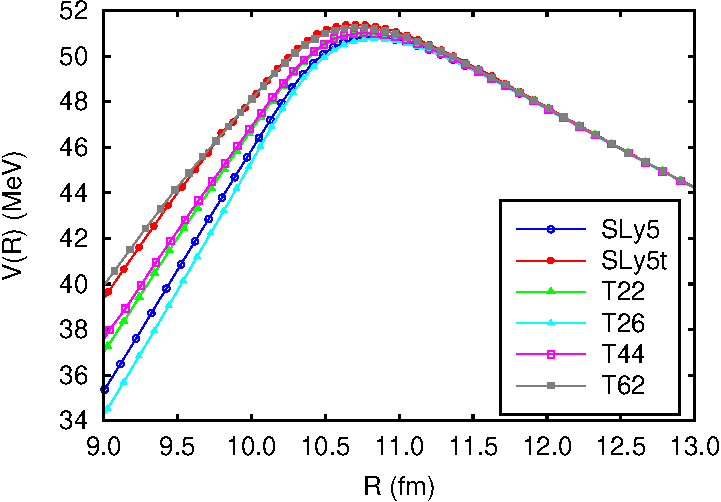
\includegraphics[width=\textwidth]{../Figures/TensorPot/V5_Ca48Ca48.pdf}
	\caption{Internuclear potential obtained from DC-TDHF approach for the reaction $^{48}\mathrm{Ca}+\mathrm{^{48}Ca}$ with SLy5, SLy5t,
		T22, T26, T44, and T62 forces.
		\label{Fig:TIJ}}
\end{figure}

Until now, the studies have utilized the tensor force SLy5t.
To obtain a comprehensive and rigorous understanding of the effects of the tensor force in heavy-ion collisions,
we now proceed to a comparison among the results of various forces, for which the coupling constants
are listed in Tab.~\ref{tab:CC}. Taking the reaction $^{48}\mathrm{Ca}+\mathrm{^{48}Ca}$ as an example,
we show the nucleus-nucleus potential with the six forces SLy5, SLy5t T22, T26, T44, and T62 in Fig.~\ref{Fig:TIJ}.
For T$22$ and T$44$ the potentials are close to each other, indicating the isoscalar tensor coupling has
negligible effect in this reaction. By comparing the results with T$26$, T$44$, and T$62$, the potential increases as the isovector tensor
coupling decreases. This clear dependence of isoscalar and isovector tensor coupling may be due to the interplay between tensor terms
and rearrangement of mean-field. The effect of the isoscalar tensor with the proton and neutron single particle spectrum moving
in the same way seems to be canceled by the refitting of the parameters.
However, the refitting does not incorporate the effect of isovector tensor in the same way.
Detailed discussions on this can be found in Ref.~\citep{Guo2018_PLB782-401}.
The T$62$ (T$26$) interaction also leads to similar potentials as SLy5t (SLy5), even though they have quite different tensor coupling constants,
because the rearrangement of the mean-field for T$62$ (T$26$)
produce additional effects which cancel part of the tensor force in SLy5t (SLy5).
\begin{figure}
	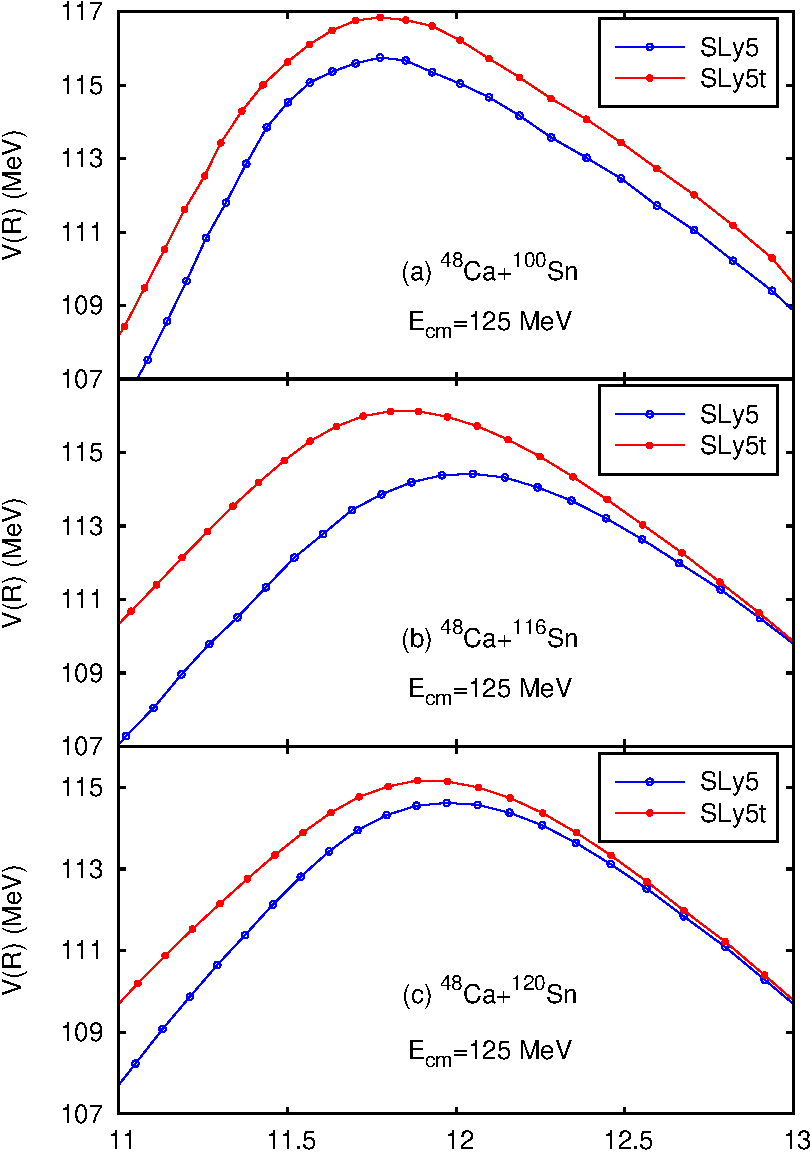
\includegraphics[width=0.9\textwidth]{../Figures/TensorPot/V4_ppt.pdf}
	\caption{Internuclear potential obtained from DC-TDHF approach for the Ca+Sn systems with SLy5 (open circle) and SLy5t (solid circle) forces.
		\label{Fig:heavy}}
\end{figure}

To gain a better insight into the tensor force, the dynamical potential is shown in Fig.~\ref{Fig:heavy} for various Ca+Sn systems
which involve one medium and
one heavy reaction partner. For $^{48}\mathrm{Ca}$, $^{100}\mathrm{Sn}$, and $^{120}\mathrm{Sn}$, the ground states are found to be spherical for
both SLy5 and SLy5t. However, the $^{116}\mathrm{Sn}$ nucleus exhibits small quadrupole deformation $\beta_2$ of 0.077 and 0.026 for SLy5 and SLy5t, respectively,
for which the deformation difference arises from the tensor force. Since the outcome of collision dynamics strongly depends on the deformation orientation
of colliding partners, the deformed nucleus $^{116}$Sn is initially set as the tip orientation in both SLy5 and SLy5t with the symmetry axis of $^{116}$Sn parallel to the internuclear axis. We find that, for the Ca+Sn systems,
the effects of the tensor force show similar trends as in the spin-unsaturated Ca+Ca, Ca+Ni, and Ni+Ni systems presented in Fig.~\ref{Fig:medium}.
The tensor force has the largest effect on the reaction $^{48}\mathrm{Ca}$+$^{116}\mathrm{Sn}$ as compared to the reactions with $^{48}\mathrm{Ca}$ colliding $^{100}\mathrm{Sn}$ and $^{120}\mathrm{Sn}$
isotopes, which may be due to the strong effect of the tensor force on the energy difference of single-proton states  $1\mathrm{h}_{11/2}$ and $1\mathrm{g}_{9/2}$ along the Z=50 isotopes for $^{116}\mathrm{Sn}$, as shown in Ref.~\citep{Colo2007_PLB646-227}.
Another suspected cause for this large effect arising from the tensor force in the $^{48}\mathrm{Ca}$+$^{116}\mathrm{Sn}$ reaction is the static deformation effects leading to a vastly different dynamical path for the system.


\section{Summary}
We incorporate the full tensor force into the FHF and DC-TDHF approaches to investigate the impact of the tensor force on heavy-ion internuclear potentials for ten representative systems in different mass regimes.
As expected we find that static potentials are systematically higher than the dynamical results, however, the variation of dynamical potential barriers induced by tensor force
is larger than those of the static case, which are attributed to the microscopic dynamical effects included in TDHF.
For light systems, the tensor force is found to have small effects on the nucleus-nucleus potential, with the barrier height and inner part of the barrier changing by a fraction of an MeV. Even this small change may lead to large effects in cross sections when considering deep sub-barrier collisions at energy scales common in astrophysical systems.
For medium and heavy spin-unsaturated reactions the effect is much more pronounced, with changes from a fraction of an MeV to almost 2~MeV for the barrier height. These differences indicate an important impact on sub-barrier fusion dynamics and a substantial fusion hindrance effect arising from the tensor force.

The fully microscopic TDHF theory has shown itself to be rich in
nuclear phenomena and continues to stimulate our understanding of nuclear dynamics.
The time-dependent mean-field studies seem to show that the dynamic evolution
builds up correlations that are not present in the static theory.
While modern Skyrme forces provide a much better description of static nuclear properties
in comparison to the earlier parametrizations, there is a need to obtain even better
parametrizations that incorporate deformation and reaction data into the fit process.
The tensor force should be a part of these investigations.
\label{summary}


\section{Acknowledgments}
%todo add acknowledgments
This work is partly supported by NSF of China (Grants No. 11175252 and 11575189),
NSFC-JSPS International Cooperation Program (Grant No. 11711540016), and Presidential Fund of UCAS,
and by the U.S. Department of Energy under grant No. DE-SC0013847.
The computations in present work have been performed on the High-performance Computing Clusters of SKLTP/ITP-CAS and
Tianhe-1A supercomputer located in the Chinese National Supercomputer Center in Tianjin.


\clearpage



%%
%% Future Work
% This is an example of the `Future work' section.
% To generate the final document, run latex, build and quick build commands
% on the skeleton-thesis file (not this one)


%%
%% Final conclusion of the dissertation
\chapter{Conclusion}
\label{sec:future_work_conclusion}
The uniting tool behind the work presented in this thesis has been the use of TDHF to explore nuclear reactions at the mean-field level.
From quasielastic scattering to the total fusion of nuclear fragments, TDHF alone can readily describe the outcome of nuclear collisions.
As mentioned before, at the base level, TDHF is optimized for the description of one-body observables~\citep{balian1981}.
This predictive ability is furthered by the development and use of extensions to the base theory to uncover correlations and effects beyond the mean-field.
It is through this effort that nuclear density functional theory has become the dominant tool in recent years to study nuclear reactions at low energies -- energy scales that are of interest to superheavy and neutron rich element formation, seed reactions of the r-process, and even the general description of equilibration in interacting quantum many-body systems.

To briefly summarize, each chapter either has focused on a specific aspect of nuclear reactions or attempts to exhaustively characterize a given system.
In Chapter~\ref{chapters:chapter_2}, I have discussed the development of a new technique to explain the impact of nucleon transfer on the fusion of heavy ions.
Through this method, we have managed to elegantly link experimental results to the fundamental process of nucleon transfer and succinctly explain the anomalous results seen in the data.
As the method developed depends only on the nuclear EDF, it may continue to be used for any future study of fusion for any reactions of interest.
Chapter~\ref{chapters:chapter_3} has also explored fusion reactions, though at a more fundamental level.
Beyond the implications of the role of the Pauli principle in heavy ion collisions, the development and implementation of the DCFHF method has provided yet another tool to apply future studies of fusion.
The DCFHF prescription is also completely general and may be used as an input for those studying fusion using theories other than our own.

Less focused on theoretical development are the projects presented in Chapters~\ref{chapters:chapter_4} and~\ref{chapters:chapter_5} which investigated the effect of the Skyrme tensor interaction on fusion probabilities for a large range of nuclei.
This sort of study is interesting, as the EDF is the only external input into a TDHF calculation, the fitting of which representing the only connection to experimental data at all.
In a similar vein is Chapter~\ref{chapters:chapter_6} which has studied the fusion probabilities of \textsuperscript{12}C+\textsuperscript{12}C at energies of astrophysical interest.
This provides vital information regarding reaction rates of carbon burning in stars, thus informing nucleosynthesis pathways in general. 

The last two chapters diverge from the narrow focus on fusion by systematically investigating transfer via two vastly different techniques.
Chapter~\ref{chapters:chapter_7} has approached the problem by using direct TDHF collisions to study what drives fragment production in $^{48}$Ca+$^{249}$Bk reactions.
Through the use of a large number of calculations for multiple orientations, a trend emerged pinning the primary cause of system separation on deformed shell effects in the light outgoing fragments.
This is significant, as similar results have been seen in studies of fission~\citep{scamps2018}, implying a deeper connection between the two processes.
Finally, Chapter~\ref{chapters:chapter_8} goes beyond TDHF to study transfer in symmetric collisions of $^{176}$Yb for multiple orientations and energies.
By peering at the distribution of particles transferred, the likelihood of fragment production can be mapped to see that the system may very well prove to be an excellent probe of the neutron rich region of the nuclear chart.
Such multinucleon transfer reactions are becoming more and more available thanks to build ups in experimental ability, and give the opportunity to look further into the properties neutron rich and superheavy nuclei.

The sum total of this work and all others in this area serves as the foundation for the next step in studying the nuclear many-body problem as it relates to reactions and structure studies.
Through further development of extensions to the base theory and as of yet unimagined approaches to better handle many-body correlations, the future of low-energy physics relies on improving our collective understanding of how systems of many particles interact with each other.
Indeed, if an end goal could be identified it would be with the complete quantum description of many-body tunneling in fission and reactions.
While the work presented in this thesis has made steps in this direction by better describing fusion and transfer mechanisms, there is still much ground to cover.

%%
%% Bibliography
\singlespacing
\bibliographystyle{mnras_formatted}
% \bibliographystyle{plainnat}
\citestyle{aa}


\bibliography{../Bibliography/bibliography}

\clearpage

%%
%% Appendices
% This is an example of the `Appendices' section.
% To generate the final document, run latex, build and quick build commands
% on the skeleton-thesis file (not this one)

\begin{appendices}

%% 1st Appendix
\chapter{Appendix A}\label{app:A}

\end{appendices}


%% End of the document
\end{document}
